\documentclass[pfe]{tnreport} % If you are in 1nd year
\usepackage{tikz}
\usepackage{amssymb}% http://ctan.org/pkg/amssymb
\usepackage{pifont}% http://ctan.org/pkg/pifont
\newcommand{\cmark}{\ding{51}}%
\newcommand{\xmark}{\ding{55}}%

\loadglsentries{glossary}

%\documentclass[stage1a,confidential]{tnreport} % If you are writing confidential report
\def\reportTitle{Mise en place d'une solution d'externalisation et de centralisation des sauvegardes} % Titre du mémoire
\def\reportLongTitle{Elaboration de plans de sauvegarde et de restauration des données} % Titre plus long du mémoire

\def\reportAuthor{Mathieu Dreyer}
\def\reportAuthorEmail{\email{mathieu.dreyer@telecomnancy.eu}} % Courriel de l'élève

\def\reportAuthorAddress{20, rue Malvina Cezard} % Adresse de l'élève
\def\reportAuthorCity{54180, HOUDEMONT} % Adresse (cont.) de l'élève
\def\reportAuthorPhone{06.14.79.73.07} % Téléphone de l'élève

\def\reportSupervisor{Frédéric Decle} % Prénom Nom de l'encadrant industriel

\def\reportCompany{LMI Solutions} % Nom de l'entreprise d'accueil
\def\reportCompanyAddress{3, rue du chapitre} % Adresse de l'entreprise
\def\reportCompanyCity{54670, MILLERY} % Adresse (cont.) de l'entreprise
\def\reportCompanyPhone{03.83.32.14.15} % Téléphone de l'entreprise
\def\reportCompanyLogoPath{figures/Logo-LMI-Solutions} % Logo de l'entreprise -- comment this definition to remove company logo

\def\place{Houdemont} % Ville pour la signature pour l'engagement anti-plagiat
\def\date{\today} % Date pour la signature de l'engagement anti-plagiat


\begin{document}

\maketitle
\pagenumbering{roman}

\insertAntiPlagiarismAgreement{Dreyer, Mathieu}{31611128}

\cleardoublepage

\makesecondtitle

\section*{Remerciements (optionnel)}
\addcontentsline{toc}{chapter}{Remerciements}

Merci à toutes les personnes qui ont contribué à la bonne réalisation de mon projet de fin d'étude et qui m'ont aidé lors de la rédaction de ce rapport.

Je tiens à remercier mon encadrant universitaire, M Olivier Airaud, pour sa disponibilité et ses conseils qui m'ont aidé tout au long de mon projet, ainsi que pour sa présence et son soutien.

J'adresse mes remerciements au gérant de l'entreprise qui a été également mon référent pendant le projet, M Frédéric Decle, pour la confiance accordée, les missions assignées et pour m'avoir permis de faire mon alternance au sein de LMI Solutions.

Je tiens aussi à remercier les personnes du service informatique de LMI Solutions pour leur aide 
et leurs précieux conseils durant le projet et pour m'avoir transmis les connaissances techniques dont j’avais besoin pour réaliser mon alternance.

Enfin, je tiens à remercier toutes les personnes qui m'ont conseillé et relu lors de la rédaction de ce rapport.


\cleardoublepage

\renewcommand{\baselinestretch}{0.5}\normalsize
\tableofcontents
\renewcommand{\baselinestretch}{1.2}\normalsize
\cleardoublepage

\pagenumbering{arabic}
\setcounter{page}{1}

\chapter{Introduction}

Aujourd'hui, le développement  de l'entreprise dépend largement de ses données informatiques. Par conséquent, il semble inévitable et urgent de protéger les entreprises grâce à une sauvegarde fiable. La sauvegarde des données est la mémoire de l'entreprise. Sans sa mémoire, à quoi ressemblerait l'entreprise ? \newline
Une sauvegarde est une sécurité en cas de problème.
Elle permet de sauvegarder la totalité des données, d’un répertoire ou d’une base de données sur un support sécurisé. \newline
En cas de dysfonctionnement ou de non disponibilité, ces données peut être restaurée afin que les services aux utilisateurs redeviennent opérationnels le plus rapidement possible, l’objectif étant d’éviter toute perte de données et d’assurer une reprise d’activité. \newline
Le but est de minimiser les conséquences associées à la perte de données informatiques. Ces conséquences peuvent avoir un impact significatif direct ou indirect sur les activités de la société. Ensuite, la sauvegarde des données permet d'éviter les pannes naturelles, les erreurs humaines, les virus ou les catastrophes.

Mais comment choisir efficacement un système de sauvegarde et comment le mettre en place et le rendre résistant aux dommages?

Ce projet a pour but d'analyser les solutions de sauvegarde, de choisir celle qui correspond le mieux aux besoins de LMI Solutions et de maquetter son utilisation.

Afin de réussir ce projet, un état de l'art des solutions existantes chez les différents clients de LMI Solutions et une analyse des meilleures solutions du marché seront effectuées, afin de pouvoir choisir trois solutions, selon différents critères. \newline
Un outil de sauvegarde sera choisi, et sera ensuite maquetté pour pouvoir être mis en place chez les différents clients.
A l'issue de cette phase, si la solution est adaptée aux besoins génériques des clients, elle sera mise en place.

L’objectif était d’implémenter une gestion centralisée des sauvegardes pour les clients de LMI Solution et devait permettre : \newline
\begin{itemize}
 \item D’avoir un suivi régulier de l’état des sauvegardes des différents serveurs pour 
s’assurer de pouvoir les restaurer en cas de besoin ; 
\item D’identifier les sauvegardes qui posent des problèmes et de pouvoir y remédier rapidement ;
\item De mettre en place de bonnes pratiques pour la gestion de ces sauvegardes, en 
fonction de la criticité des données à protéger (plan de sauvegarde, sauvegarde hebdomadaire ou
quotidiennes, ...) ;
\item Tester régulièrement qu'une sauvegarde est possible dans des délais compatibles avec les 
exigences des différents clients. \newline 
\end{itemize}

\clearpage


\chapter{Besoins et objectifs du projet}

\section{Contexte, périmètre et enjeux}

Dans le monde actuel, les entreprises ont de plus en plus besoin de conserver des données, en cas de dysfonctionnement. \newline
Comme la grande majorité des entreprises disposent de serveurs contenant leurs données, il est donc nécessaire de les conserver. Le but étant de pouvoir retrouver facilement des données perdues, effacées, ou corrompues. \newline
LMI Solutions se positionne en tant que société de service pour différents clients incluant la mise en place de solutions adaptées à leurs besoins. \newline
Il est important de connaître l'enjeu des sauvegardes pour une entreprise. En informatique, plusieurs éléments peuvent être source de perte de données : \newline
\begin{itemize}
 \item Erreur humaine : mauvaise manipulation, suppression de données;
 \item Vol de données : un mauvais accès à des données;
 \item Virus : tout type de virus qui bloque l'accès aux données;
 \item Obsolescence : matériel informatique qui est usé, durée de vie atteinte. \newline
\end{itemize} 

Tous ces risques peuvent donc provoquer une perte de données au sein des entreprises. \newline
En effet, prenons comme exemple le récent incendie du datacenter d'OVH à Strasbourg. Une grande partie des serveurs a brûlé, ce qui a entraîné une perte d'informations. Les entreprises qui ne disposaient pas d'une sauvegarde de données ont eu des difficultés à reprendre leur activité (récupération manuelle) ou même une impossibilité de reprendre l'activité (perte de commandes clients, perte de chiffre d'affaires, etc..). \newpage 
Une perte de données représente, en moyenne pour une entreprise : \newline
\begin{itemize}
 \item Pour les victimes de cyber-attaques ou de vol de données, leur réputation, leur fidélité et la confiance des clients sont considérablement réduites (baisse de chiffre d'affaire, de revenus, etc..) ;
 \item La perte de données engendre souvent une perte de clients ;
 \item Une baisse d'activité, voire un arrêt d'activité.\newline
\end{itemize} 
Après que plusieurs clients aient subi des attaques de cryptolocker, ce qui est à l'origine de perte de données ou de temps d'arrêt conséquent et compte tenu de l'importance de la situation de l'entreprise (risque de perte de clients...), mon tuteur m'a demandé de lui fournir une solution de sauvegarde sécurisée et centralisée. \newline
Un cryptolocker est le nom d'un malware de type verrouillage de chiffrement, un cheval de Troie dont le but est d'exécuter un ransomware et d'attaquer les ordinateurs avec un système d'exploitation Windows installé. \newline
Il se propage par e-mail principalement. Lorsque le cheval de Troie est activé, il utilise un cryptage à clé publique et privée pour crypter plusieurs fichiers sur la cible. \newline
Une fois que tous les fichiers sur l'ordinateur sont infectés, il commencera à se propager à travers le réseau local pour infecter toutes les postes, serveurs possibles. Ensuite, la clé pour déverrouiller l'assemblage est uniquement stockée sur le serveur hébergeant le malware. \newline
Le virus affiche alors un message indiquant que pour déchiffrer les informations, le paiement doit être envoyé. \newline
Le paiement peut être effectué avec des coupons Bitcoin ou en espèces. Le montant demandé est valable jusqu'à une certaine date et augmentera si le paiement n'est pas effectué à temps. \newline

Pour pallier à cela, il est donc nécessaire de mettre en place un outil de sauvegarde, limitant le temps d'inactivité de l'entreprise. \newline
Actuellement, l'application Veeam Backup est déployée par LMI Solutions. \newline
C'est la meilleure solution du marché. En effet, elle propose un large panel de fonctions et s'adapte aux différentes structures. Veeam travaille sur l'ensemble des domaines de sauvegarde tandis que ses concurrents se spécialisent sur un seul domaine de sauvegarde en général, ce qui fait de Veeam Backup une solution complète et adaptée à l'ensemble des problèmes pouvant être rencontrés.\newline
Cependant, elle présente quelques problèmes pour LMI Solutions. En effet, les responsables des sauvegardes doivent se connecter de manière quotidienne sur les serveurs afin de vérifier leur état. \newline Un outils a été mis en place afin d'avoir un rapport journalier, mais celui-ci n'est pas totalement fiable. \newline
Elle propose une solution d'externalisation, qui demande du temps à mettre en place et à configurer pour chaque client. \newline
Les besoins sont : \newline
\begin{itemize}
 \item Connaître les concurrents de la solution actuelle et s'assurer qu'elle est toujours adaptée;
 \item Identifier les besoins afin de protéger les clients contre les pertes de données;
 \item Analyse des outils et produits disponibles sur le marché ;
 \item Trouver une solution pour la centralisation et la visibilité de l'état des sauvegardes;
 \item Rédiger des plans de sauvegarde à valider par les clients. \newline
\end{itemize}
Les principaux aspects du projet sont les suivants : \newline
\begin{itemize}
 \item Il faut trouver une solution répondant aux différents critères de réussite d'un projet afin d'atteindre et de respecter les différents objectifs fixés par mon tuteur; 
 \item Le rôle de responsable du bon fonctionnement de la centralisation des sauvegardes des différents clients;
 \item Pour tout achat et demande d’investissement, je devrai avoir l’accord du gérant de LMI Solutions. \newline
\end{itemize}

Les points suivants ne font pas partie du périmètre du projet : \newline

\begin{itemize}
 \item Les interventions de prestataires externes sur le matériel de LMI Solutions.
 \item La sauvegarde des applicatifs métiers.
\end{itemize}
\newpage
\section{Critères d'évaluation du projet}

Plusieurs critères ont été définis au sein de LMI Solutions permettant de statuer sur la réussite ou l'échec du projet.

\begin{table}[!h]
 \centering
 \begin{tabular}{|p{7cm}|p{5cm}|p{4cm}|}
 \hline Objectifs & Solutions envisagées & Échéances\\
 \hline Analyse fonctionnelle : Comprendre le fonctionnement des sauvegardes, le moyen de mise en place. & Documentation, plan de fonctionnement. & 30 avril 2021.\\
  \hline Évolutivité : capacité d’évolution et d’insertion de nouveaux équipements. & La capacité d'évolution de la solution proposée sera présentée. & 3 juin 2021. \\
 \hline Procédure et documentation : création de procédure et document pour une reprise et/ou suivi d'activité. & Rédaction de procédure, document de formation et de préparation à la reprise d'activité seront rédigés. & 14 juillet 2021\\
 \hline Contrôle automatique quotidien : notifications, gestion d'erreur. & Mise en place d'un modèle pour automatiser le déploiement des sauvegardes, mise en place de notifications par mail et suivi de l'état des serveurs. & 14 juillet 2021. \\
\hline Être capable de proposer des axes d’amélioration. & Une solution Cloud hybride (stockage des sauvegardes sur site et dans le Cloud) a été proposée et est étudiée par l’entreprise. & 31 juillet 2021. \\
 \hline 
 \end{tabular}
 \caption{Tableau des critères de validation du projet}
 \label{tab:critere}
\end{table}

Le tableau \ref{tab:critere} permet de regrouper l'ensemble des crtières d'évaluation du projet au sein de LMI Solutions. \newline
Il a été validé par l'ensemble de l'équipe. \newline



\chapter{Présentation du projet}

Dans cette partie les différents acteurs du projet seront présentés. \newline
Ensuite, les différents documents qui m'ont servi à mettre en place une gestion de projet seront présentés, avec leurs utilités.

\section{L'équipe}

L'équipe du projet est constituée de cinq personnes : \newline
\begin{itemize}
 \item Frédéric Decle, gérant de LMI Solutions, qui sera présent aux différentes réunions et qui validera les décisions ;
 \item Alexandre Petitcolas, qui est le responsable des sauvegardes des clients de LMI Solutions;
 \item Dominique Tougne, responsable des sauvegardes dans une zone géographique différente ;
 \item Julien Hottier, qui s'occupe des différents problèmes concernant les sauvegardes ;
 \item Mathieu Dreyer, apprenti et chef de projet. \newline
\end{itemize}

Lors des différentes réunions, au moins le gérant de l'entreprise, une personne de la partie technique et moi-même seront présents.

\section{Gestion de projet}

Le déroulement du projet se découpe en plusieurs étapes. Il est important d'abord de bien comprendre le fonctionnement des sauvegardes et les différents types avant de choisir une solution. \newline
Ainsi, la première partie portera sur une analyse des sauvegardes, avec un état de l'art et le choix d'une solution adaptée aux besoins. La seconde concernera le maquettage et la mise en place de l'outil retenu. \newline
Un outil de ticket développé par l'entreprise est mis en place à LMI Solutions, qui permet d'avoir un suivi sur chaque projet. \newline
Il s'agit d'un outil de ticket, développée par l'entreprise. Chaque jour, mes tâches ont été saisies, ce qui permet à chaque collaborateur relié à la tâche de pouvoir suivre mon avancée. \newline

\subsection{Matrice RACI}

Une partie importante du projet à ne pas sous-estimer est la partie concernant les relations humaines. Dans 
un projet il y a toujours des parties prenantes internes et externes, et savoir bien organiser la 
communication avec toutes les parties est un point important. En premier lieu j’ai identifié toutes les 
parties qui étaient liées de près ou de loin au projet grâce à une matrice RACI, qui m’a permis de définir 
les responsabilités de chaque acteur du projet. Cela permettra de définir quel acteur est affecté à quelle tâche, afin d'éviter une redondance des rôles. \newline
La variante RASCI a été utilisée, afin de définir les différents supports du projet et les personnes consultées pour des questionnements.

\begin{figure}[ht]
 \centering
 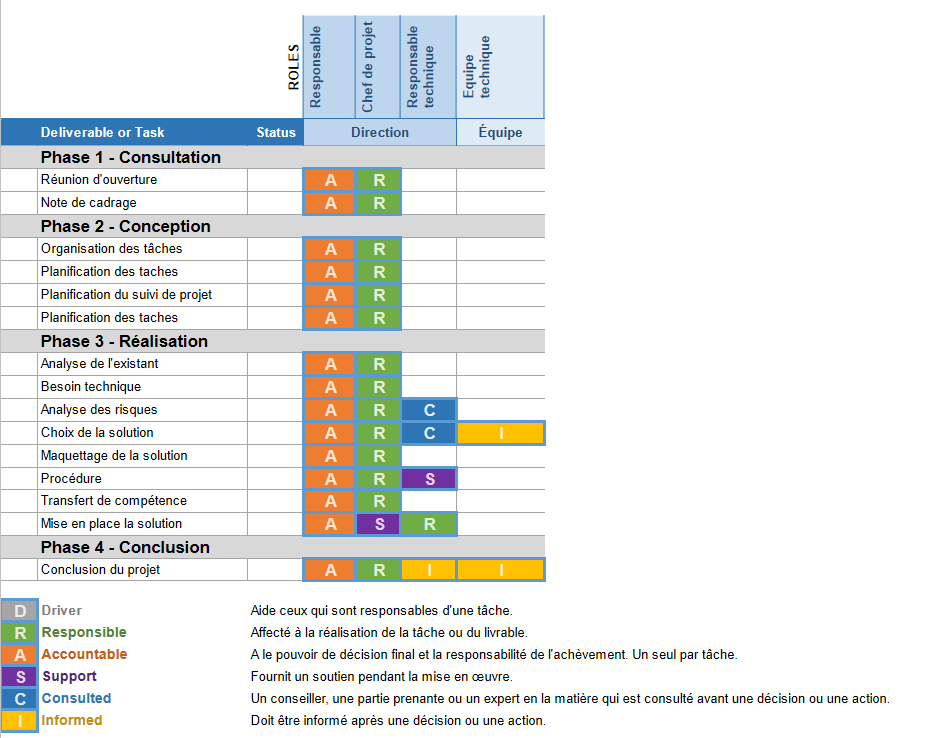
\includegraphics[width=18cm]{figures/raci.png}
 \caption{Matrice RACI}
 \label{fig:raci}
\end{figure}

La matrice \ref{fig:raci} représente les différentes phases du projet, avec les différents tâches et les acteurs de celles ci. \newline
Mais la partie humaine ne se limite pas à identifier les parties prenantes, il faut savoir communiquer avec chaque acteur du projet au bon moment, il est donc utile également de faire des points régulièrement.

\subsection{Diagramme de Gantt}

Une gestion de projet a été mise en place afin d'avoir un certain recul sur celui-ci. \newline
Celle ci est constituée d'un diagramme de Gantt, afin de pouvoir définir des dates clés et de permettre aux différents acteurs d'avoir une vision sur l'avancée de ce projet. \newline
Cela permet de définir un planning réaliste, tout en visualisant les complexités. Il aide également à mettre en place une certaine communication avec l'équipe. \newline
Un autre avantage d'un tel diagramme est qu'il permet d'être modifié de manière simple en cas d'évènement inattendu. En effet, chaque tâche est planifiée sur une durée, donc si l'acteur de la tâche se rend compte que celle ci nécessite plus de temps, il est possible de le moduler facilement. \newline
Pour le diagramme, l'outil Microsoft Project et un outil en ligne permettant de créer et de partager des diagrammes sans compte ont été utilisés.
\begin{figure}[ht]
 \centering
 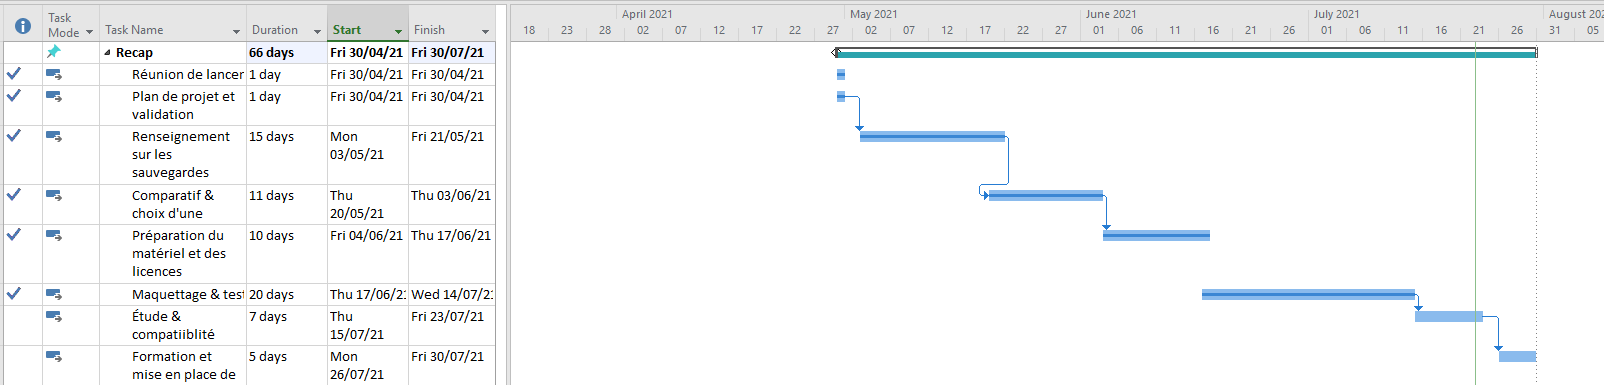
\includegraphics[width=18cm]{figures/gantt.png}
 \caption{Diagramme de Gantt}
 \label{fig:gantt}
\end{figure}

Le diagramme \ref{fig:gantt} illustre les durées estimées des différentes tâches. Il s'agit de la version finale, avec les modifications qui ont eu lieu au cours du projet. En effet, entre la première version et la version finale du diagramme, différents points ont nécessité plus de temps. 

Le découpage du projet a été fait de cette manière : \newline
\begin{itemize}
 \item Le choix d'une solution, avec la rédaction d'un document comparatif et les échanges avec l'équipe technique pour statuer sur un outil;
 \item La préparation du matériel et des licences nécessaires, qui signifie faire un descriptif du matériel nécessaire et des licences, ainsi que de la commande et la livraison de ces derniers;
 \item Le maquettage de la solution, avec une série de tests pour vérifier son application au sein des clients;
 \item La rédaction des documents nécessaires pour la mise en place chez le client et pour former les différents acteurs à la solution choisie;
 \item La mise en place de l'outil au sein d'un client, ou de plusieurs clients, en fonction des besoins clients et des limites de la solution. \newline
\end{itemize}


\begin{figure}[ht]
 \centering
 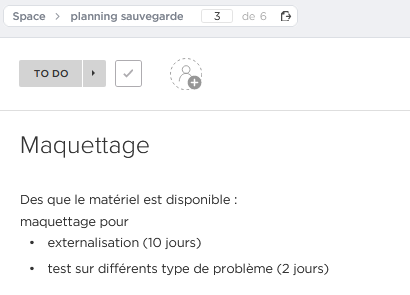
\includegraphics[width=7cm]{figures/ganttv2.png}
 \caption{Sous tâche dans le diagramme de Gantt}
 \label{fig:ganttcapt}
\end{figure}
\newpage
Chaque découpage est constitué de sous tâches, avec une durée estimée, comme le représente la capture d'écran ~\ref{fig:ganttcapt}. Il a été effectué de la manière suivante : \newline
\begin{itemize}
    \item Choix d'une solution, avec la recherche, la rédaction d'un document explicatif, la soumission de l'analyse des solutions à M. Decle et la réunion finale afin de choisir une solution. Cette partie doit être effectuée pour le 3 juin 2021 ; \newline
    \item La préparation du matériel, qui comprend le descriptif du matériel nécessaire pour réaliser le maquettage et également un descriptif des licences nécessaires et la commande et livraison du matériel. Cette phase doit être finalisée pour 17 juin ; \newline
    \item La partie procédure, qui comprend la rédaction des différents documents (plan de sauvegarde, procédure d'installation). La date butoir est définie le 14 juillet ; \newline
     \item L'étude des clients, constituée d'une analyse sur les besoins et la compatibilité entre la solution choisie et ces besoins, pour le 23 juillet afin de mettre en place chez un client ensuite; \newline
     \item La mise en place, avec la formation des personnes qui interviendront sur le projet sur la semaine du 30 juillet. \newline
\end{itemize}


Chaque semaine, un point est réalisé avec mon tuteur et avec l'équipe technique. \newline
A chaque fin de tâche, un mail est envoyé pour informer les différents acteurs du projet de son avancée. \newline
De plus, chaque document rédigé est partagé sur le drive de l'équipe, ce qui permet de suivre l'avancée totale du projet. \newline
\newpage
\subsection{Analyse fonctionnelle}

Une analyse fonctionnelle du projet a été effectuée, avec la méthode APTE (APplication aux Techniques d'Entreprise). \newline
Il s'agit d'une méthodologie pratique, rapide à mettre en place et visuelle. \newline
Elle permet de transformer les besoins des clients sous forme de fonctions à atteindre.

La première étape de cette méthode consiste à identifier : \newline
\begin{itemize}
 \item Produit : Que voulons-nous concevoir ?
 \item Clients : Quelles personnes utilisent des produits et bénéficient de services ?
 \item Matériaux de travail : Qu'est-ce qui affectera les produits et services ?
 \item Besoin de répondre : Quel est le but de la conception de nos produits ? \newline
\end{itemize}

Du point de vue graphique, il peut être représenté sous la forme d'une « bête à cornes ». En effet, dans des projets informatiques, il est important de bien définir le besoin avant de se lancer dans sa conception. 
\begin{figure}[!h]
 \centering
 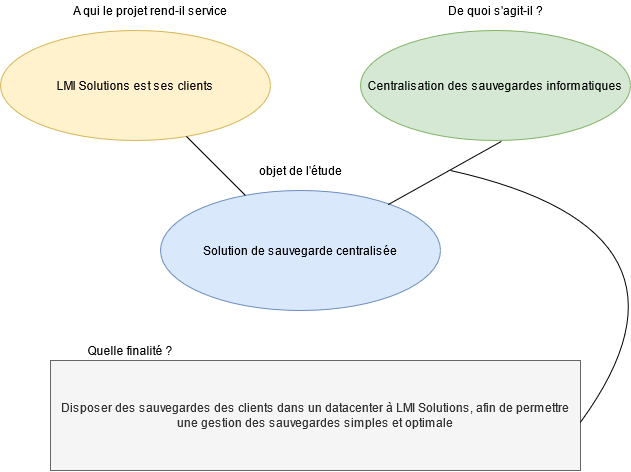
\includegraphics[width=15cm]{figures/bull(1).png}
 \caption{Diagramme de bête à corne simple}
 \label{fig:beteacorne}
\end{figure}
\newpage
Par conséquent, dans la figure ~\ref{fig:beteacorne}, nous avons : \newline
\begin{itemize}
 \item Produit : Une solution de sauvegarde externalisée ;
 \item Clients : Aux différents clients de LMI Solutions et à l'entreprise ;
 \item Matériel : Sauvegardes informatiques ;
 \item Besoins à satisfaire : Permettre d'externaliser les sauvegardes à LMI \item Solutions pour les rendre accessibles, rendant la gestion plus simple et optimale. \newline
\end{itemize}

Il permet de distinguer l'utilité de la conception d'un produit.

Avec ce graphique, une liste des fonctions a été effectuée. Deux types de fonctions ont été déterminées : \newline
\begin{itemize}
 \item la ou les fonctions principales (FP) : ce sont les raisons d'être du produit, celles qui lui permettent de remplir les objectifs ;
 \item les fonctions contraintes (FC) : ce sont les caractéristiques du produit qui sont imposées par son environnement. \newline
\end{itemize}

J'ai réalisé un diagramme de pieuvre, permettant de trouver les différentes fonctions. \newline
Ce genre de diagramme définit le lien entre le système et son environnement. Le schéma identifie la plupart des fonctions du système.

\begin{figure}[ht]
 \centering
 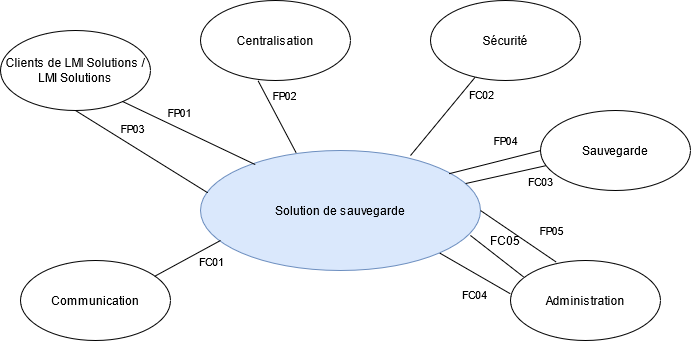
\includegraphics[width=15cm]{figures/peiuvre.png}
 \caption{Diagramme de pieuvre}
 \label{fig:pieuvre}
\end{figure}
Les fonctions principales sont les suivantes : \newline
\begin{itemize}
    \item \textbf{FP01} : Le système permet d'externaliser les sauvegardes. \newline
Il faut que les sauvegardes soient externalisées, de manière régulière, vers un serveur hors site du client.\newline
\item \textbf{FP02} : Le système permet de centraliser les sauvegardes. \newline
La solution doit être capable de regrouper l'ensemble des sauvegardes sur un même serveur, afin d'avoir accès à toutes les sauvegardes depuis un serveur. \newline
\item \textbf{FP03} : Le système permet de gérer les incidents. \newline
Depuis l'outil, les différents incidents (erreurs de sauvegardes, serveur indisponible) doivent être corrigibles. \newline
\item \textbf{FP04} : Le système permet un suivi de l'état des sauvegardes. \newline
La solution doit permettre aux techniciens d'avoir un rapport sur l'état des sauvegardes, de manière simple et explicite. \newline
\item \textbf{FP05} : Le système permet un déploiement rapide. \newline
Il faut que le déploiement de l'outil chez un client se fasse de manière rapide, en moins de 20 minutes. \newline
\end{itemize}
Les fonctions contraintes sont les suivantes : \newline
\begin{itemize}
\item \textbf{FC01} : Le système doit disposer d'une gestion d'alerte. \newline
En cas de dysfonctionnement, il faut être alerté. \newline
\item \textbf{FC02} : Le système doit présenter des méthodes de sécurité face aux ransomwares. 
Il faut que l'outil propose une fonction permettant d'augmenter la sécurité face aux virus. \newline
\item \textbf{FC03} : Le système doit réaliser des sauvegardes. 
\newline Des sauvegardes seront effectuées avec l'outil de manière régulière, il est donc nécessaire qu'il propose une fonction de sauvegarde. \newline
\item \textbf{FC04} : Le système doit être supervisé.
la solution doit permettre d'être alerté en cas de problème sur un serveur de sauvegarde (espace de stockage, inaccessible..). \newline
\item \textbf{FC05} : Le système doit disposer d'une console de management.
Il doit être possible d'accéder à l'ensemble des sauvegardes depuis l'outil. \newline
\end{itemize}

Suite à cette analyse fonctionnelle, il est important de définir les risques du projet. \newpage

\subsection{Analyse des risques}

D'un point de vue organisationnel, un autre aspect important est la gestion des risques.\newline
Tout projet comporte des risques qui doivent être activement identifiés et gérés. \newline
Le risque est une combinaison de probabilité et de gravité. Le niveau de risque préliminaire peut être fourni dans l'analyse des dangers. Il faut déterminer la vérification, la prédiction plus précise et l'acceptation du risque dans l'évaluation des risques. L'objectif principal des deux est de fournir la meilleure méthode pour contrôler ou éliminer les risques. \newline
Pour cela, j'ai utilisé une matrice de gestion des risques : pour me préparer aux différents risques que je pourrais rencontrer tout au long du projet. 

\begin{figure}[!h]
 \centering
 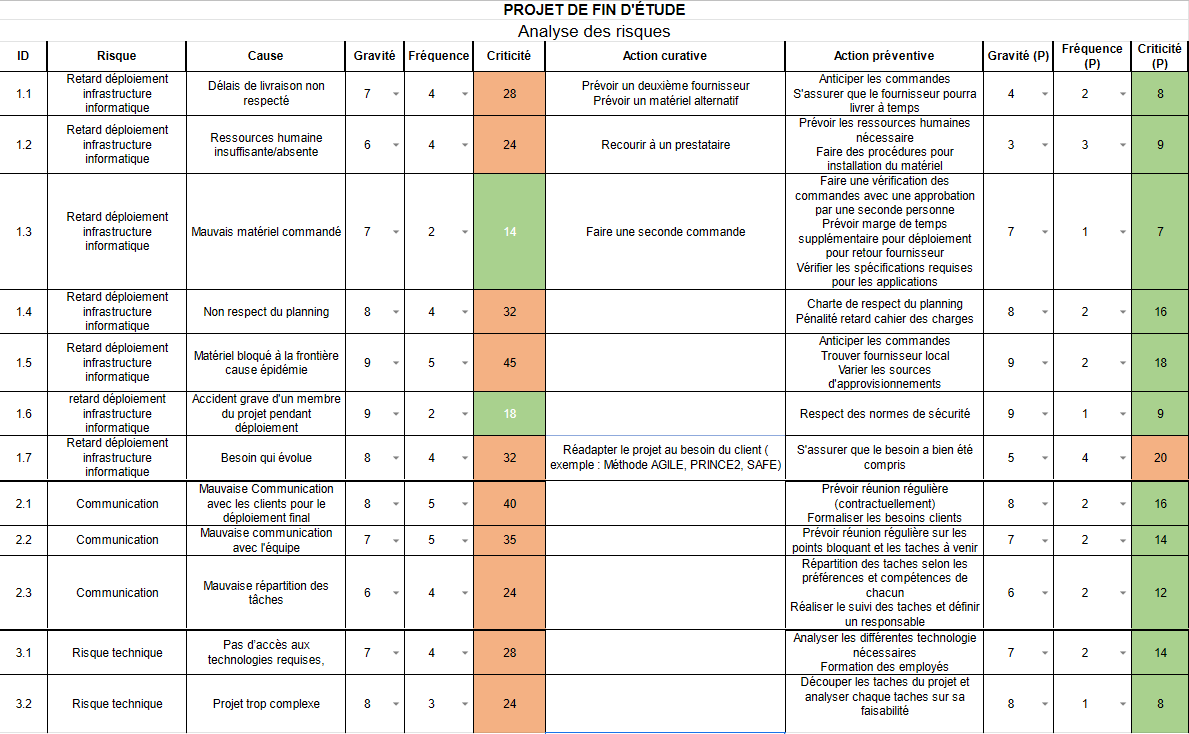
\includegraphics[width=17cm]{figures/risques.png}
 \caption{Analyse des risques}
 \label{fig:risk}
\end{figure}

Comme le montre le diagramme des risques \ref{fig:risk}, plusieurs risques ont été mis en exergue. Pour les anticiper au mieux, des actions préventives ont été définies afin d'éviter de se retrouver dans un cas critique. Elles sont présentes dans l'analyse des risques, suivi des taux modifiés grâce à ces actions. \newline
Par exemple, pour éviter une mauvaise commande du matériel, l'action préventive est la suivante : Faire une vérification des commandes avec une approbation par une seconde personne et prévoir une marge de temps supplémentaire pour le déploiement. Avant la criticité de la tâche était de 14, contre 7 après l'action corrective. \newline
Maintenant que la gestion de projet a été définie, nous pouvons passer à l'analyse du fonctionnement des sauvegardes.
\chapter{Analyse des sauvegardes}
Cette partie permettra de comprendre le fonctionnement des sauvegardes. Elle sera composée d'un état des lieux actuel, des différentes méthodologies existantes, du choix d'une méthodologie et d'un mode de sauvegarde.

\section{État des lieux de la sauvegarde}

Pour répondre au mieux à la problématique, il faut au préalable effectuer une analyse de ce qui est déjà en place au sein des établissements des différents clients, avec le type de sauvegarde et la solution choisie.
Afin de réaliser un état de l'art à jour, une vérification a été effectuée pour chaque client qui possède une solution de sauvegarde. 

\subsection{Infrastructure présente chez les clients}

Avant de faire l'inventaire de ce qui est en place chez les différents clients, il faut comprendre le fonctionnement de ces derniers.
Pour nos clients, l'infrastructure fonctionne de la manière suivante : les données sont situées sur un serveur, et chaque personne y accède à distance. La majorité des applications et des données se trouvent sur les lecteurs réseaux. \newline
Le but de la sauvegarde pour ces clients est donc de conserver les données sur les serveurs.
Les types de serveurs sont les suivants : \newline
\begin{itemize}
 \item Serveur de données, qui contient différents espaces de stockages partagés en fonction des permissions;
 \item Serveur avec connexion bureau à distance (RDP), qui regroupe les différentes applications utilisées par l'entreprise;
 \item Serveur contrôleur de domaine, serveur qui répond aux demandes d'authentification de sécurité dans un domaine de réseau informatique;
 \item D'autre serveurs, qui varient en fonction des besoins clients. \newline
\end{itemize}
 Il sera donc nécessaire de sauvegarder les différents serveurs du client. \newline
 Le but étant de limiter au maximum le temps d'arrêt d'une entreprise lors d'un problème survenant sur un ou plusieurs serveurs.
 
De manière générale, l'infrastructure est donc constituée d'un serveur physique, avec un ensemble de machines virtuelles qui servent à remplir différents rôles nécessaires pour le client.


\subsection{Inventaire des sauvegardes}

Afin d'avoir une liste des outils de sauvegarde présent chez les clients, il m'a fallu me connecter sur les serveurs des différentes entreprises et échanger avec la partie technique qui a mis en place les solutions. \newline
Pendant la récupération de ces données, j'ai rédigé un document permettant de recenser les stratégies misent en place. \newline
\begin{figure}[ht]
 \centering
 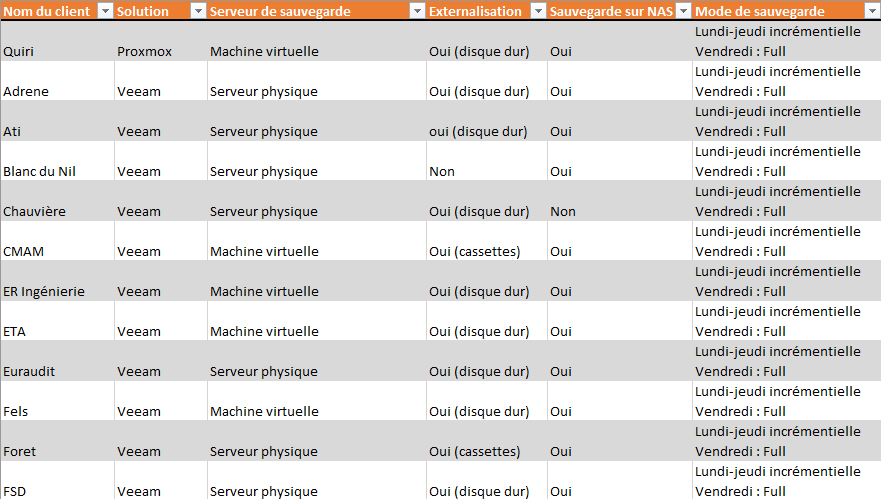
\includegraphics[width=17cm]{figures/etatclient.png}
 \caption{Listing des solutions de sauvegarde}
 \label{fig:etatclient}
\end{figure}

Le tableau ~\ref{fig:etatclient} représente l'état actuel des solutions de sauvegarde chez les clients de LMI Solutions.

Ce document représente les informations essentielles de la sauvegarde mise en place. \newline Il contient les informations sur : \newline
\begin{itemize}
 \item L'outil de sauvegarde (Veeam, Arcserv, etc..);
 \item L'état du serveur de sauvegarde (physique ou virtuel);
 \item Les supports de sauvegarde externe (disque dur, cassettes, etc..);
 \item La présence ou non de sauvegarde sur NAS;
 \item Le type de sauvegarde (incrémentale, complète, etc..).\newline
\end{itemize} 

Grâce à ces informations, nous remarquons un type de configuration présent dans la majorité des infrastructures. \newline
Celui ci est constitué de la solution Veeam, d'une sauvegarde de type incrémentiel, avec une sauvegarde sur support externe et sur NAS. \newline
Une réunion a été effectuée à l'issue de la rédaction de ce document avec la partie technique, afin de comprendre les besoins et les raisons de ce type de fonctionnement. \newline
La sauvegarde de type incrémentiel permet de sauvegarder plus de données, en consommant moins d'espace. Ce type de sauvegarde sera décrit dans la partie suivante du rapport. \newline
Le fait de conserver les sauvegardes sur plusieurs supports permet d'augmenter la sécurité des données. \newline 
L'externalisation des sauvegardes va donc permettre d'ajouter une sécurité supplémentaire en permettant à LMI Solutions de les gérer.

\subsection{Analyse de chaque sauvegarde}

Les sauvegardes de chaque client sont différentes, en fonction de la version de l'outil, de l'heure de sauvegarde et d'autres paramètres. \newline
\begin{figure}[ht]
 \centering
 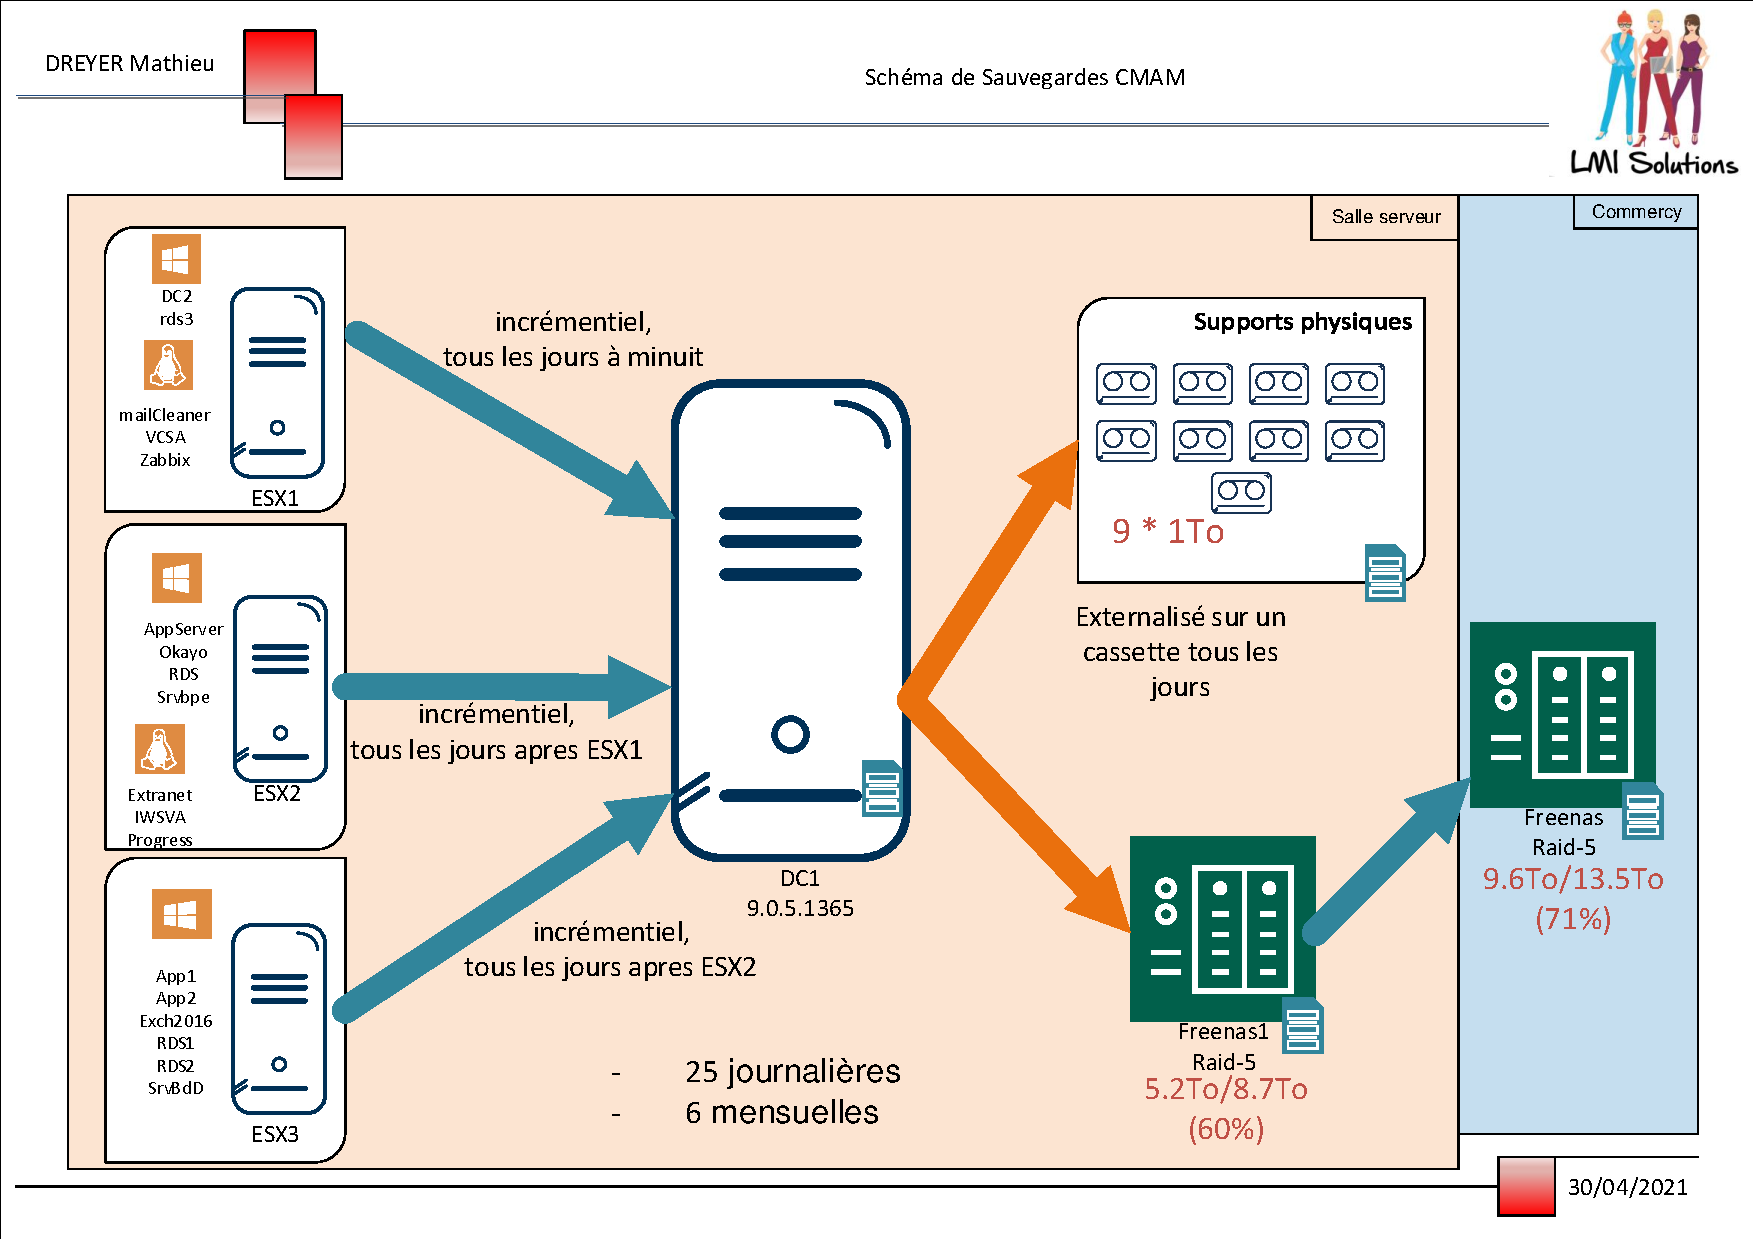
\includegraphics[width=18cm]{figures/schemaclient.pdf}
 \caption{Exemple d'un schéma de sauvegarde}
 \label{fig:schemaclient}
\end{figure}
Il existe des schémas représentant l'infrastructure des clients, mais ils datent du déploiement de la solution. Ils n'ont pas été mis à jour au fur et à mesure des années. \newline
Pour permettre à l'équipe technique de connaître rapidement le fonctionnement des sauvegardes au sein des différents clients, j'ai réalisé un schéma pour chacun d'entre eux, mentionnant toutes les informations nécessaires. \newline
Il faut également que ce document soit modifiable facilement au cours des années par l'équipe, afin de le garder à jour. \newline
J'ai donc utilisé l'outil Visio de Microsoft. Il s'agit d'un outil connu par l'ensemble de l'équipe et qui prend en charge les versions antérieures. \newline
La figure ~\ref{fig:schemaclient} est un exemple de schéma réalisé. \newline
Un modèle générique a été choisi et présenté à l'équipe pour l'appliquer au sein des différents clients. \newline
Le but est de pouvoir rapidement distinguer les éléments de chaque client, sans avoir à lire l'entièreté du schéma. \newpage
Les informations essentielles sont les suivantes : \newline
\begin{itemize}
 \item L'outil de sauvegarde et sa version;
 \item Connaître si la sauvegarde est externalisée;
 \item La volumétrie disponible sur les différents supports lors de la réalisation du schéma;
 \item Les serveurs sauvegardés.\newline
\end{itemize} 
Un code couleur est également appliqué pour des équipements qui se situent à des emplacements distincts.
Grâce à ce document, les principales données concernant les sauvegardes sont accessibles rapidement.
Une vingtaine de schémas a été réalisée, pour pouvoir statuer sur les différents états des sauvegardes chez les clients.
Grâce à l'état de l'art actuel et aux différents schémas, il est possible de décrire un type de sauvegarde mis en place au sein de la majorité des clients de LMI Solutions. \newline
Pour un grand nombre d'entre eux, il s'agit d'une sauvegarde des serveurs, comme les données se situent sur les différents serveurs. \newline
Les sauvegardes sont effectuées sur des plages horaires en dehors de l'activité de l'entreprise, pour ne pas ralentir l'accès aux données et aux serveurs. \newline
La plupart des clients ont comme solution un NAS de sauvegarde et une externalisation des sauvegardes sur disque dur, cassette ou dans un cloud. \newline
Les serveurs de sauvegarde ne font pas partie du domaine de l'entreprise cliente, pour éviter que des virus tels que les ransomwares se répandent sur ces derniers.
\section{Étude des sauvegardes}

Il existe différentes façons de sauvegarder les données d'une entreprise. \newline
Afin d'apporter une analyse complète et une solution au projet, il m'a été essentiel d'étudier les différentes méthodes et solutions existantes qui répondent au problème et d'en proposer à LMI Solutions. \newline

\subsection{État de l'art des solutions existantes}
Afin de planifier et de former l'équipe technique sur une solution, il m'a fallu au préalable comprendre les nuances des solutions de sauvegardes.

\begin{figure}[ht]
 \centering
 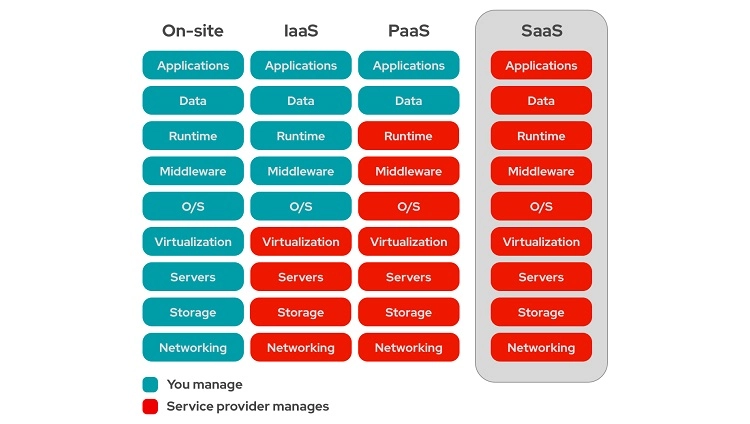
\includegraphics[width=19cm]{figures/comparatif_sauvegarde.png}
 \caption{Regroupement des types de solutions, source 
 \href{https://www.redhat.com/en/topics/cloud-computing/public-cloud-vs-private-cloud-and-hybrid-cloud}{Redhat}}
 \label{fig:famille}
\end{figure}
Pour pouvoir les comparer, il faut d'abord les trier par catégorie, afin de trouver quelle catégorie répond le mieux aux besoins et ensuite quelles solutions sont les meilleures dans ce type de sauvegarde. \newline


Il existe quatre familles de sauvegardes, qui sont représentées sur la figure \ref{fig:famille}. \newline
Chaque famille permet une gestion différente des sauvegardes. \newline Afin de savoir quel type correspond le mieux aux besoins de LMI Solutions, chacun d'entre eux va être défini.

La catégorie On-Site : il s'agit d'une copie en temps réel des différentes données sur un serveur ou sur un support externe (disque dur ou autre). Il existe plusieurs solutions, telles que: Veeam, Syncback, Cobian Backup ou même Cloud Station.\newline
Elles permettent de copier automatiquement les données après la détection des modifications dans le dossier de travail. \newline
Une autre solution s'effectue avec un système de RAID1, qui permet de cloner tous les disques en temps réel. Il n'y a pas de logiciel dans la gestion de RAID.\newline

Le Cloud service est une infrastructure, une plate-forme ou un logiciel hébergé par un fournisseur tiers, qui peut être fourni aux utilisateurs via Internet.\newline
Il existe trois principaux types de solutions de service: \glsxtrfull{IaaS}, \glsxtrfull{PaaS} et \glsxtrfull{SaaS}. \newline
Chacun de ces types sera détaillé dans les parties suivantes. \newline
Tout cela facilite le flux des données utilisateur du client frontal via Internet vers le système du fournisseur de services Cloud.

l'\glsxtrfull{IaaS} : il s'agit d'une forme de Cloud computing qui vous permet d'externaliser l'infrastructure informatique matérielle dans un environnement virtualisé.\newline
Les utilisateurs peuvent y accéder via des API ou des tableaux de bord et louent essentiellement une infrastructure. \newline
L'utilisateur gère des éléments tels que les systèmes d'exploitation, les applications et les intergiciels, tandis que le vendeur est responsable de la maintenance du matériel, des réseaux, des disques durs, du stockage de données et des serveurs.

Le \glsxtrfull{PaaS}, de l'anglais \textit{plateform as service} est un type de Cloud computing, principalement destiné aux développeurs ou aux sociétés de développement. \newline
Ce type de Cloud suit le fonctionnement suivant : le matériel et une plate-forme logicielle d'application sont fournis et gérés par un fournisseur de services en Cloud externe. \newline
L'utilisateur gère les applications qui s'exécutent au-dessus de la plate-forme et les données sur lesquelles l'application repose.

Le \glsxtrfull{SaaS} est un modèle de distribution de logiciels dans lequel des fournisseurs tiers hébergent des applications et les fournissent aux clients sur Internet. \newline
En règle générale, les applications \glsxtrfull{SaaS} sont des applications Web ou des applications mobiles auxquelles les utilisateurs peuvent accéder via un navigateur Web. \newline
\subsection{Choix du type de sauvegarde}

Dans le cas de nos clients, il faut sauvegarder des données sur les différents serveurs. \newline
Chacun des types de sauvegarde précédemment étudié est utile dans un cas particulier. \newline
Suite à différentes recherches et échanges avec la partie technique de LMI, le but est d'être le prestataire de sauvegarde des données du client. Cela signifie qu'il faut que l'entreprise s'occupe de la sauvegarde au niveau des serveurs. \newline
Les sauvegardes de la famille du service de cloud correspondent plus à des entreprises qui veulent gérer elles-mêmes leurs données. \newline
Le type de sauvegarde qui correspond au besoin de LMI Solutions est On-site, avec une gestion de la sauvegarde des applications aux serveurs. \newline
Il faut également prendre en compte qu'une copie hors site sera effectuée, mais cela reste dans la catégorie "On-Site" comme LMI Solutions s'occupera de l'ensemble des sauvegardes. 

\section{Méthodologie de sauvegardes}

Il existe différentes façons d'effectuer une sauvegarde. \newline
Le but de celles-ci, dans le cas de nos clients, est de pouvoir sauvegarder les données et de limiter au maximum le temps d'arrêt lorsqu'un problème survient. \newline
Pour ce projet, la recherche sera centrée sur les quatre méthodes courantes de sauvegarde qui sont : la sauvegarde complète, la sauvegarde différentielle, la sauvegarde incrémentale et la sauvegarde miroir. Ensuite, une comparaison de chacune de ces sauvegardes va être effectuée, afin de pouvoir choisir le type de sauvegarde le plus adapté pour chaque client.

\subsection{Sauvegarde complète} 

\begin{figure}[ht]
 \centering
 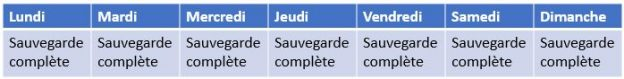
\includegraphics[width=15cm]{figures/complete-624x79.jpg}
 \caption{Tableau récapitulatif du fonctionnement de la sauvegarde complète, source
 \href{https://all-it-network.com/types-sauvegarde/}{it-network}}
 \label{fig:complete}
\end{figure}
Le tableau \ref{fig:complete} illustre un planning de sauvegarde avec la méthodologie complète. Ici, une sauvegarde complète est effectuée chaque jour. \newline
Il s'agit d'une méthode de type «annuler» et «remplacer». Le contenu de la sauvegarde sera écrasé par de nouvelles informations. Si le volume est important, c'est une méthode très sûre mais qui nécessite du temps. Il est donc recommandé de la planifier le soir pour ne pas empêcher les utilisateurs de travailler le lendemain matin. \newline
Ce type de sauvegarde comprend la totalité des données (fichiers, répertoires et sous-répertoires) sélectionnées à un instant T donné, et le placement du tout sur le support de sauvegarde. \newline 
Il faut comprendre que si la même tâche est relancée après deux jours et qu'il n'y a pas de modification du fichier d'origine, la sauvegarde sera la même que la précédente. \newline
Pour la restauration, il suffit de prendre la dernière sauvegarde. \newline
Dans le cas où il est nécessaire de conserver d'anciennes sauvegardes, ce système a particulièrement besoin d'espace de stockage. \newline
L'utilisation de ce type de sauvegarde n'est pas non plus une tâche facile, car pour chaque sauvegarde, l'ensemble des données est récupéré, qu'il soit modifié ou non. \newline
Cependant, il est possible de supprimer toutes les anciennes sauvegardes et d'en conserver qu'une seule.\newline
Ce type est le plus simple à mettre en œuvre. 
\subsection{Sauvegarde différentielle}

Il s'agit d'une méthode de sauvegarde de toutes les informations qui ont changées depuis la dernière sauvegarde complète. \newline
\begin{figure}[!h]
 \centering
 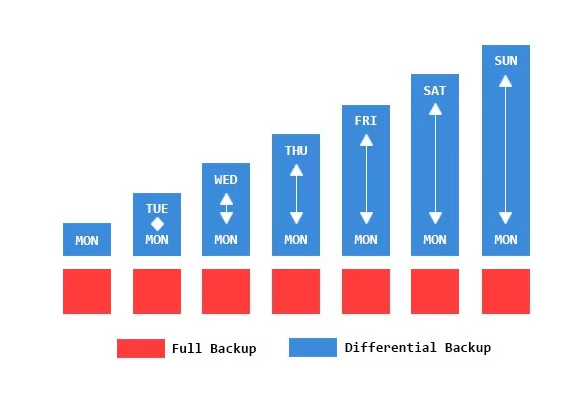
\includegraphics[width=15cm]{figures/differentiel.png}
 \caption{Tableau récapitulatif du fonctionnement de la sauvegarde différentielle, source
 \href{https://www.dz-techs.com/fr/compare-the-different-backup-types}{DzTech}}
 \label{fig:differentielle}
\end{figure}

La première sauvegarde sera exécutée en tant que sauvegarde complète. La deuxième sauvegarde effectuée le jour J +1 ne contiendra que les fichiers modifiés par rapport au contenu de la première sauvegarde (jour J).\newline
Le tableau \ref{fig:differentielle} montre un planning de sauvegarde différentielle. \newline
Dans ce mode de fonctionnement, une sauvegarde complète est effectuée un certain jour et des sauvegardes différentielles les autres. \newline
Pour lancer une restauration, il faut avoir à sa disposition la première sauvegarde et la dernière sauvegarde. La sauvegarde intermédiaire, c'est-à-dire la sauvegarde entre la première sauvegarde et la dernière sauvegarde, peut être supprimée. \newline
Il est également possible de les conserver. Cela permet de retrouver des copies de fichiers enregistrés à une date précise, et donc d'avoir accès à chaque donnée. \newline
Plus ce genre de sauvegarde est effectué, plus cela prendra de temps. La comparaison des fichiers se fait toujours avec la première sauvegarde. \newline
Afin de raccourcir la durée de fonctionnement, il est nécessaire de refaire une sauvegarde complète de manière périodique.

\subsection{Sauvegarde incrémentale}

Cette méthode, incrémentale ou incrémentielle, ne sauvegarde que les informations qui ont changées depuis que la dernière sauvegarde a été enregistrée sur le support. \newline
\begin{figure}[ht]
 \centering
 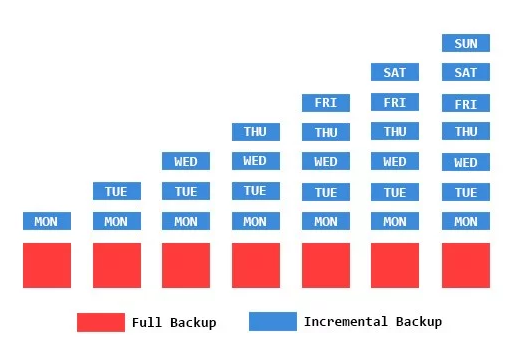
\includegraphics[width=15cm]{figures/incremental.png}
 \caption{Tableau récapitulatif du fonctionnement de la sauvegarde incrémentale, source
 \href{https://all-it-network.com/types-sauvegarde/}{dzTechs}}
 \label{fig:incrementale}
\end{figure}

La première sauvegarde a été exécutée en tant que sauvegarde complète. Par exemple, en prenant le jour J comme base de référence, la deuxième sauvegarde est effectuée le jour J +1 (jour suivant, ou prochain jour programmé de sauvegarde), le logiciel de sauvegarde vérifiera quels fichiers ont été modifiés. \newline Par conséquent, seuls les fichiers modifiés seront pris en compte dans la deuxième sauvegarde. 
Le troisième jour, le programme créera une copie de sauvegarde des modifications apportées depuis le deuxième jour. \newline
Chaque sauvegarde est faite par rapport à la précédente. Il est donc nécessaire de disposer de toutes les sauvegardes pour restaurer.\newline
Avec le planning \ref{fig:incrementale}, on peut qu'il s'agit d'un mode de fonctionnement semblable au précédent. Les sauvegardes différentielles sont remplacées par des incrémentales. \newline
La sauvegarde suivante utilise le même principe.\newline En d'autres termes, le processus de sauvegarde de fichiers prend en compte tous les éléments qui ont changé depuis la dernière sauvegarde. \newline
Ce qui différencie donc la sauvegarde incrémentale et la différentielle est la sauvegarde de comparaison. Dans celle ci, on se base sur la dernière sauvegarde, or dans la différentielle, il s'agit de la dernière sauvegarde complète qui est utilisée. \newline
Par conséquent, le système est très rapide et occupe très peu d'espace de stockage. \newline
D'un autre côté, puisque toutes les sauvegardes sont nécessaires, le processus de restauration est lent. En effet, la recherche du dernier fichier modifié conduit à la manipulation et à l'étude de toutes les autres sauvegardes différentes.
\subsection{Sauvegarde miroir}

Une sauvegarde miroir est une copie exacte des données source vers un autre support. La différence avec une sauvegarde complète est que les données sont compressées. \newline
Lors de l'utilisation de la mise en miroir, une seule sauvegarde contient les fichiers système qui existaient lors de la dernière sauvegarde. \newline Cette méthode est souvent utilisée en parallèle d'une autre méthode, comme il est facile de perdre un fichier avec celle ci. En effet, lorsqu'une modification est effectuées sur les données, elle s'effectue également sur la sauvegarde miroir. Si un fichier est supprimé, il le sera aussi sur la sauvegarde.  \newline
Cette méthodologie n'est donc pas applicable à LMI Solutions et est écartée. \newline
En effet, le fait de ne pas pouvoir disposer des anciens fichiers est bloquant pour les clients en cas d'erreur (suppression, fichier corrompu..). \newline
Elle sera néanmoins utilisée dans le comparatif, afin de distinguer ses avantages et inconvénients. \newpage

\subsection{Comparatif des méthodologies}

Afin de savoir quelle sauvegarde correspond le mieux aux clients, il faut également analyser les avantages et inconvénients de chacune de ces méthodes de sauvegarde.

\begin{table}[!h]
 \centering
 \begin{tabular}{|p{4cm}|p{6cm}|p{6cm}|}
 \hline
 Type de sauvegarde & Avantages & Inconvénients\\
 \hline
 Complète & Simple à mettre en place, option simple pour retrouver les données & Temps de sauvegarde lent, restaurations lentes\\
 \hline
 Différentielle & Restauration rapide & Coûteux en stockage, plus le nombre de sauvegarde est important, plus la sauvegarde sera lente \\ 
 \hline
 Incrémentale & Rapidité de sauvegarde, peu coûteuse en stockage & Restauration plus lente \\
 \hline Miroir & Restauration rapide et ne contient pas de fichiers obsolètes & Pas de possibilité de restaurer d'anciens fichiers \\
 \hline 
 \end{tabular}
 \caption{Tableau comparatif des différents types de sauvegarde}
 \label{tab:comparatif_type}
\end{table}

Suite à cette analyse, il est maintenant possible de sélectionner un type de sauvegarde. \newline
Le tableau \ref{tab:comparatif_type} représente les avantages et inconvénients de chaque méthode. \newline
D'abord, comme la sauvegarde complète est lente et demande beaucoup d'espace, celle ci va être plus coûteuse en espace de stockage pour les clients, et nécessitera un temps d'arrêt conséquent. \newline
Ensuite, la sauvegarde différentielle permet une restauration rapide, mais sera également plus coûteuse pour les clients. Cependant, les clients ont besoin d'une sauvegarde journalière. \newline
En effet, la majorité des clients disposent de nombreux fichiers, qui sont modifiés chaque jour. Il faut donc les sauvegarder de manière journalière, sans perdre les différentes versions de ces derniers. Pour cette raison, la sauvegarde différentielle ne sera pas retenue dans notre cas. \newline
La sauvegarde incrémentale, quant à elle, correspond le mieux à nos besoins, avec un coût de stockage plus faible que les autres sauvegardes, donc elle représente un investissement plus faible pour le client. La restauration sera plus lente que la sauvegarde différentielle, mais les sauvegardes seront faites de manière plus rapide, ce qui ne bloquera pas les utilisateurs. \newline L'avantage également de ce type de sauvegarde est qu'il permet de restaurer avec seulement une sauvegarde complète et une différentielle. \newpage
\section{Études des solutions}

Grâce à l'analyse des méthodes de sauvegarde réalisée précédemment, cette partie portera donc sur les solutions de sauvegarde du type "On-Site".

Afin de choisir au mieux un outil de sauvegarde, une analyse des solutions existantes sera faite. \newline
Pour se faire, la recherche a été découpée en deux parties : \newline
- La première, qui consiste en une étude des principales solutions sur le marché ;\newline
- La seconde, qui sera un comparatif entre celles ci.

\subsection{Les solutions sur le marché}

Suite à différentes analyses, il est possible d'avoir une liste des principales solutions qui sont les plus utilisées. Sur le graphique ci dessous, nous pouvons voir les différentes solutions ainsi que leur classement dans différents domaines. 
\begin{figure}[ht]
 \centering
 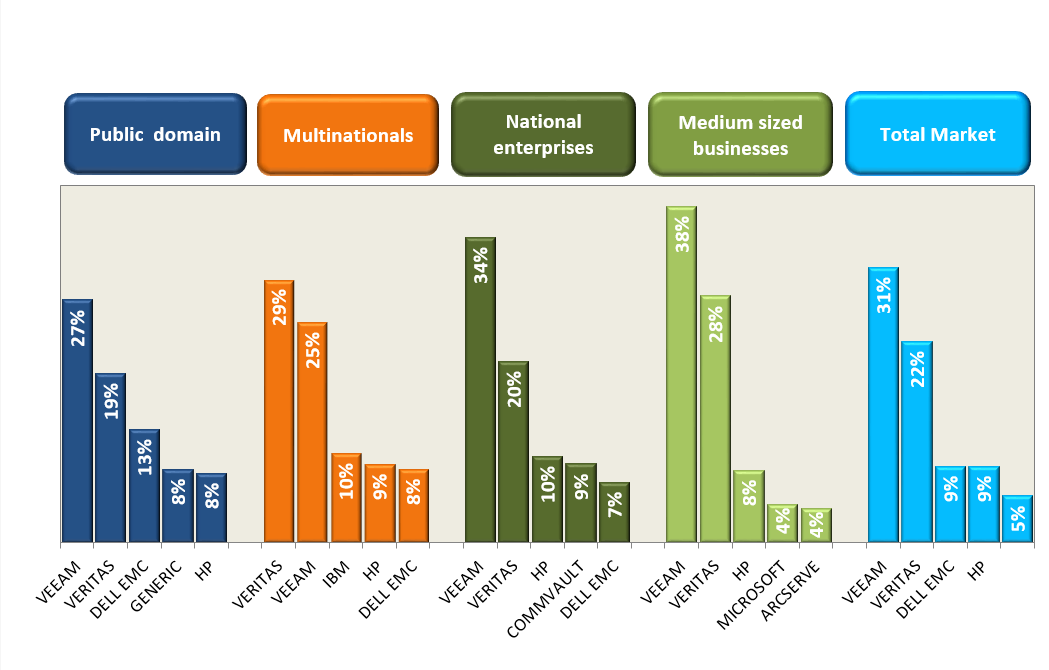
\includegraphics[width=15cm]{figures/Backup.png}
 \caption{Graphique représentant la position des solutions, source
 \href{https://www.smartprofile.io/analytics-papers/veeam-big-winner-in-back-up-software/}{smartprofile}}
 \label{fig:backup_state}
\end{figure}

La figure \ref{fig:backup_state} représente les principales solutions sur le marché. Parmi celles-ci, des solutions ont déjà étés mise en place à LMI Solutions, mais n'ont pas été conservés suite à différents problèmes rencontrés. \newline
J'ai donc choisi de prendre les solutions qui ne sont pas connues de LMI Solutions et qui se positionnent en première position dans un domaine. \newline
Ensuite, une analyse sera faite sur les solutions qui évoluent depuis les dernières années. \newline
Le but est de trouver un outil qui permet de faire des sauvegardes de manière externalisée. Il faut également que le logiciel propose un tarif égal ou inférieur à Veeam qui est actuellement mise en place. \newline
Enfin, une grande partie des clients de LMI Solutions sont des petites et moyennes structures, il faut donc que l'applicatif soit adapté aux besoins de ce type de structure. \newline
Avec ces informations, certaines solutions ont pu être écartées. Pour le comparatif, cinq solutions sont retenues. \newline

\subsection{Choix d'une solution}

Le choix d'une solution se fera parmi les suivantes : \newline
\begin{itemize}
 \item Veeam, actuellement mise en place; \newline
 \item Veritas qui est l'outil le plus utilisé dans les multinationales; \newline
 \item Altaro qui se positionne sur les infrastructures avec un rôle par serveur. Elle évolue beaucoup depuis quelques années et propose de nouvelles fonctionnalités au cours du temps; \newline
 \item Commvault, software de sauvegarde regroupant de nombreuses fonctions ; \newline 
 \item Acronis, outil performant dans le domaine de la reprise d'activité après un incident. \newline
\end{itemize}

La comparaison se fera sur les éléments principaux nécessaires pour les clients de LMI Solutions, à savoir la rapidité de récupération, la possibilité de copier les données hors-site, la sécurisation des sauvegardes et la disponibilité sur les différents logiciels.

\begin{table}[!h]
 \centering
 \begin{tabular}{|p{5cm}|p{1.5cm}|p{2cm}|p{1.5cm}|p{1.5cm}|p{1.5cm}|}
 \hline Fonctions & Veeam & Commvault & Acronis & Veritas & Altaro\\
 \hline Fonctionne sans agent & \cmark & \cmark & \cmark & \xmark & \xmark \\
 \hline Réplication de VM & \cmark & \cmark & \cmark & \xmark & \cmark \\
 \hline Récupération de VM instantanée & \cmark & \xmark & \xmark & \cmark & \cmark \\
 \hline Copies inaltérables
 pour la protection anti-ransomwares & \cmark & \xmark & \cmark & \cmark & \cmark \\
 \hline Backup serveurs physiques & \cmark & \cmark & \cmark & \cmark & \cmark \\
 \hline Backup pour vmware et hyper-v & \cmark & \cmark & \cmark & \xmark & \cmark \\
 \hline Récupération de fichiers & systèmes & \cmark & nécessite un agent & avec sélection & \cmark \\
 \hline Accélération intégrée du WAN & \cmark & limitée & \xmark & limitée & \cmark \\
 \hline Supporte les cassettes & \cmark & \xmark & \xmark & \cmark & \xmark \\
 \hline 
 \end{tabular}
 \caption{Tableau comparatif des solutions de sauvegarde}
 \label{tab:comparatif_solution}
\end{table}
Le tableau \ref{tab:comparatif_solution} met en évidence les points essentiels qu'un outil de sauvegarde doit posséder. Il permet de voir les fonctions manquantes ou présentes dans une solution. \newline
Suite à cette analyse, il est possible d'écarter des solutions. L'agent lui n'est pas contraignant, cependant il est important de le noter pour en avoir connaissance. \newline
Veritas ne propose pas la réplication de machine virtuelle, seulement de la restauration. \newline
Acronis ne permet pas de faire de la récupération instantanée, ce qui est un point bloquant. \newline 
En effet, le but de la solution de sauvegarde et de permettre un accès rapide en cas de problème aux différents serveurs. \newline
Les trois solutions suivantes, CommVault, Veeam et Altaro, ont donc été soumises à l'équipe pour en choisir une à mettre en place. \newline
Une réunion a été planifiée afin de choisir un outil pour le déploiement. \newline
Au cours de celle-ci, chacune des trois solutions a été présentée, avec ses principales fonctionnalités. \newline
Un comparatif a également été effectué sur les fonctions principales et les contraintes. \newline
\begin{table}[!h]
 \centering
 \begin{tabular}{|p{7cm}|p{2cm}|p{2cm}|p{2cm}|}
 \hline Fonctions principales et contraintes & CommVault & Veeam & Altaro \\
 \hline Le système permet d'externaliser les sauvegardes & \cmark & \cmark & \cmark \\
 \hline Le système permet de centraliser les sauvegardes & \cmark & \cmark & \cmark\\
 \hline Le système permet de gérer les incidents & \cmark & \cmark & \cmark \\
 \hline Le système permet un suivi de l'état des sauvegardes & \cmark & \cmark & \cmark\\
 \hline Le système permet un déploiement rapide & \xmark & \xmark & \cmark \\
 \hline Le système doit disposer d'une gestion d'alerte et de notification & \cmark & \cmark & \cmark \\
 \hline Le système doit présenter des méthodes de sécurité face aux ransomwares & \xmark & \cmark & \cmark \\
 \hline Le système doit être supervisé & \cmark & \xmark & \cmark \\
 \hline Le système doit disposer d'une console de management & \xmark & \xmark & \cmark \\
 \hline
 \end{tabular}
 \caption{Tableau récapitulant les fonctions principales et contraintes}
 \label{tab:comparatif_Fonction}
\end{table}
\newline Afin de choisir convenablement la solution, un tableau comparatif \ref{tab:comparatif_Fonction} a été réalisé en se basant sur l'analyse fonctionnelle précédente. \newline
Le comparatif a permis de déceler les fonctionnalités essentielles pour la solution de sauvegarde, en fonction des besoins de LMI Solutions. 
Actuellement, Veeam est mise en place. Elle est leader du marché, mais se révèle avoir un tarif conséquent. \newline Ceci s'explique par le nombre de fonctionnalités qu'elle offre. 
Avec la crise sanitaire, le télé-travail est de plus en plus présent. \newline
Ceci entraîne un nombre plus important d'attaques sur les serveurs. \newline
Les clients de LMI Solutions sont sujets à des ransomwares. Il faut donc une solution qui protège au maximum l'infrastructure des entreprises contre ce genre de virus. La solution CommVault a donc été écartée des choix, en respect des fonctions définies. \newline
Lors de la comparaison entre Veeam et Altaro, nous avons pu mettre en exergue que les fonctions essentielles sont présentes dans les deux outils. \newline
Altaro se démarque des autres solutions, par son prix qui est moins élevé que celui de ses concurrents. \newline
Suite à cette réunion, l'outil Altaro a donc été sélectionnée pour être maquetté. \newline
\newpage
\section{Maquettage}

Pour maquetter la solution, il faut représenter une architecture commune des clients. \newline
J'ai choisi de prendre une infrastructure répandue chez les entreprises clientes de LMI Solutions.

\begin{figure}[ht]
 \centering
 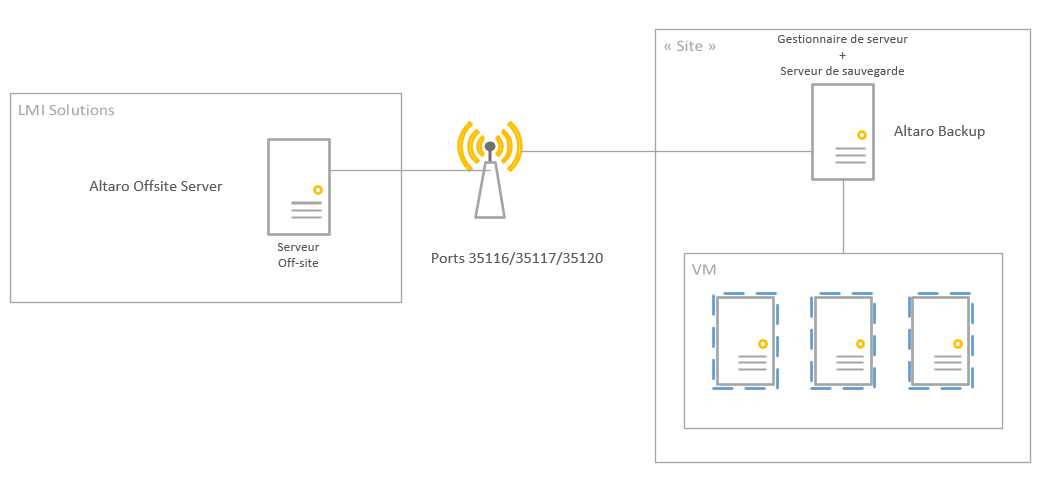
\includegraphics[width=15cm]{figures/maquette.png}
 \caption{Maquettage de Altaro}
 \label{fig:maquettage}
\end{figure}
En effet, la majorité des clients disposent d'un serveur physique, avec une multitude de serveurs virtuels. \newline
L'infrastructure sera composée d'un serveur client et d'un serveur externe comme le présente le schéma \ref{fig:maquettage}.\newline
Le premier serveur servira de gestionnaire de serveur, comportant plusieurs machines virtuelles. Sur ce serveur, l'outil Altaro Backup sera installé et une sauvegarde des différents serveurs virtuels sera mise en place. \newline
Le second serveur sera situé sur un autre réseau que le premier, afin de mettre en place une copie des sauvegardes hors site de manière régulière, sans passer par le réseau LAN. Sur celui ci, l'application Altaro Offsite Server sera installée. \newline
Le maquettage a ensuite été présenté à l'équipe technique de LMI pour validation. \newline
Une réunion a été planifiée afin de voir les axes d'améliorations possibles du maquettage. \newline
Une fois que le maquettage a été validé, il m'a fallu faire un listing du matériel pour le maquettage. \newline
Celui a donc été revu, afin de pouvoir tester les différentes options nécessaires aux différents clients.

\begin{figure}[ht]
 \centering
 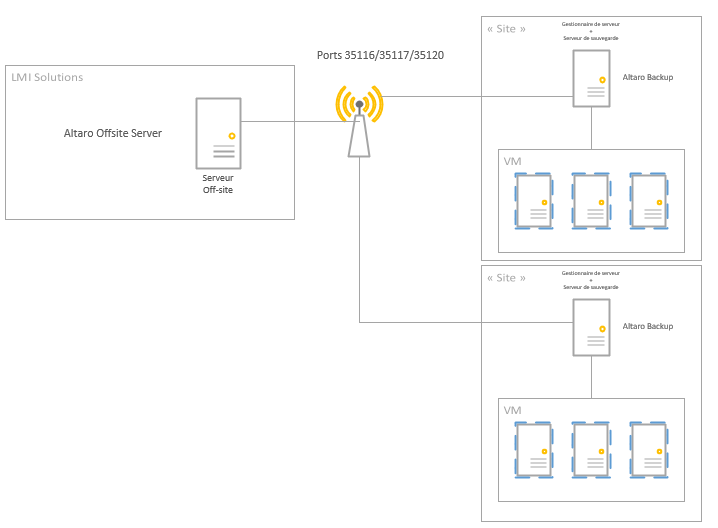
\includegraphics[width=15cm]{figures/maquettagev2.png}
 \caption{Maquettage de Altaro suite à la réunion}
 \label{fig:maquettage_v2}
\end{figure}
Le schéma \ref{fig:maquettage_v2} représente l'infrastructure à mettre en place. \newline
Le maquettage sera fait avec deux serveurs de virtualisation et un serveur hors site. Le but étant de tester la restauration d'une machine virtuelle sur un hôte différent.

Suite à cette réunion, le maquettage a été validé. \newline
Avec la crise sanitaire, une liste du matériel a été effectuée à l'issue de cette réunion, pour avoir le matériel nécessaire dans les meilleurs délais. \newline

J'ai donc choisi de prendre une infrastructure similaire aux solutions que LMI met en place chez ses clients. \newline
Les deux serveurs de virtualisations seront donc sous Windows, avec deux versions différentes, afin de tester la compatibilité. Le premier disposera d'un système d'exploitation sous Windows Server 2019, le second sera sous Windows Server 2012. \newline
Sur les deux serveurs, le système de virtualisation Microsoft Hyper-V sera installé. \newline
Ensuite, plusieurs VM seront créées, afin de pouvoir simuler une infrastructure d'entreprise. \newline
Les serveurs virtuels auront différents rôles attribués : \newline
\begin{itemize}
 \item Un serveur de gestion d'active directory;
 \item Un serveur DNS / DHCP;
 \item Un serveur proxy sous Linux. \newline
\end{itemize}

Altaro se découpe en deux outils : l'outil off-site serveur, qui permet de réaliser des copies hors site, avec la création de compte et d'accès et Altaro Backup Server, qui permet de sauvegarder les différents serveurs, . 
Sur le second serveur, la solution Altaro off-site Server sera mise en place, dans le but d'externaliser les sauvegardes réalisées. \newline 
Ce serveur se trouve à LMI Solutions. Pour mettre en place le fonctionnement, il disposera d'une IP fixe sur le réseau LAN pour mettre en place une redirection de ports sur le réseau public, afin que les données puissent arriver sur le serveur.

En parallèle du maquettage, une procédure d'installation a été rédigée, afin de faciliter les futures installations.\newline
Celle-ci explique comment installer le logiciel, la configuration pour les sauvegardes sur site et hors site.

Lors du maquettage, différents tests ont pu être mis en place. Ils permettent de définir si la solution est adaptée aux clients et permet de répondre aux besoins de LMI Solutions. \newline
Afin de s'assurer que la solution corresponde aux attentes, j'ai rédigé une fiche contenant une série de tests à effectuer. Cette fiche a été transmise aux différents acteurs du projet, pour validation.

\subsection{Test sur les fonctionnalités}


Afin de connaître les points forts et les points faibles de Altaro, les fonctionnalités ont été testées. \newline
Premièrement, des tests ont été effectués sur la version gratuite. Avec cette version, il est possible uniquement d'effectuer une sauvegarde, de la restaurer entièrement sur le même hôte ne prenant en compte que les machines virtuelles.\newline 
En comparaison avec la version gratuite de Veeam, celle ci est moins complète. Veeam permet de faire des sauvegardes complètes et gratuites de postes informatiques. \newline

\begin{figure}[ht]
 \centering
 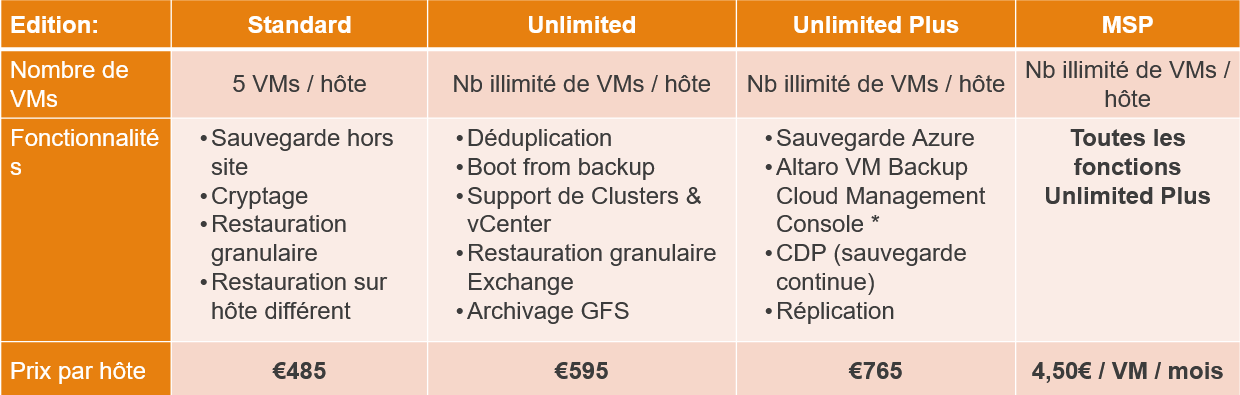
\includegraphics[width=15cm]{figures/price.png}
 \caption{Tableau récapitulatif des prix}
 \label{fig:altaro_price}
\end{figure}
La grille de tarification de Altaro dépend de l'offre ou du nombre de serveurs. \newline
Les prix affichés sur le tableau \ref{fig:altaro_price} sont sur 3 ans, sauf pour l'offre MSP qui est facturée chaque mois en fonction du nombre de serveurs. \newline
Dans les offres sont compris les mises à jour et un accès au support qui est joignable en continu, 24 heures sur 24. Ce support est un support situé dans un autre pays que la France, mais n'est pas soumis aux changements de fuseau horaire grâce à sa disponibilité. Les échanges avec le support se font en anglais uniquement. \newline 
Au niveau de l'application, celle-ci n'est pas faite sur une base SQL. \newline 
Elle consomme moins de ressource que Veeam. \newpage
L'application est rapide à installer et ne demande pas beaucoup de paramétrage. L'interface est simplifiée au maximum.\newline
\begin{figure}[ht]
 \centering
 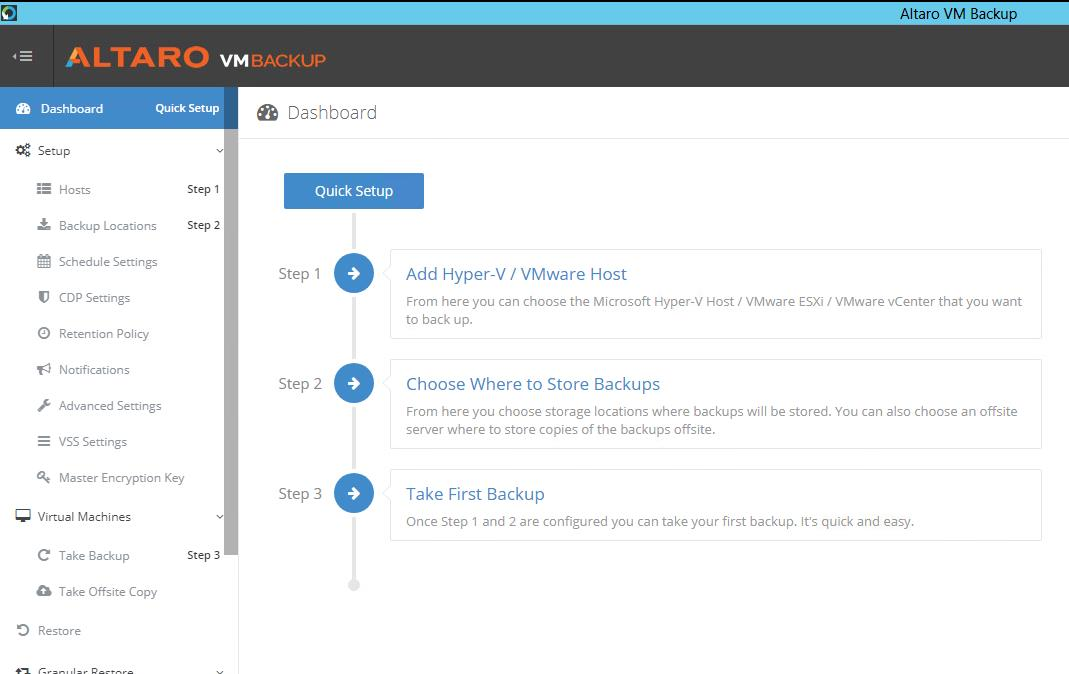
\includegraphics[width=15cm]{figures/Configure-Altaro-VM-backup-for-VMware-1.jpg}
 \caption{Capture d'écran de l'application}
 \label{fig:altaro_install}
\end{figure}
La figure \ref{fig:altaro_install} représente l'interface au premier lancement. Elle est simple à comprendre.\newline
L'outil est donc facilement utilisable. \newline
A l'issue de ces premiers tests, j'ai décidé d'appeler le fournisseur français de la solution, afin d'avoir des informations complémentaires et une licence NFR. Cette licence est une version intégrale des solutions logicielles qui permettent d’appréhender, de pratiquer et d’utiliser, pour un usage interne, toutes les fonctionnalités des logiciels proposés à la vente. \newline
Suite à l'échange téléphonique avec le revendeur français, j'ai planifié une conférence via Teams avec l'équipe technique et l'entreprise fournisseuse d'Altaro. \newline 
Le but de cette réunion est de pouvoir répondre à toutes les questions concernant la solution, pour éviter d'installer une solution que nous ne maîtrisons pas totalement. \newline
Pour préparer la réunion, j'ai mis en place une série de tests avec la licence fournie. \newline
Pour se faire, j'ai reproduit le scénario sur lequel LMI Solutions se positionne afin d'aider ses clients, à savoir un serveur Hyper-V disposant de plusieurs serveurs virtuels. \newline
J'ai effectué une sauvegarde à 17h30 des différents serveurs pendant une semaine. \newline
Lors de la première sauvegarde, l'outil demande une clé de chiffrement, pour sécuriser les sauvegardes. Il faut conserver cette clé, car elle n'est pas enregistrée. Si elle est perdue, les sauvegardes avec cette clé seront inutilisables. \newline
Ensuite, il est possible de choisir l'emplacement des sauvegardes.\newline
\begin{figure}[ht]
 \centering
 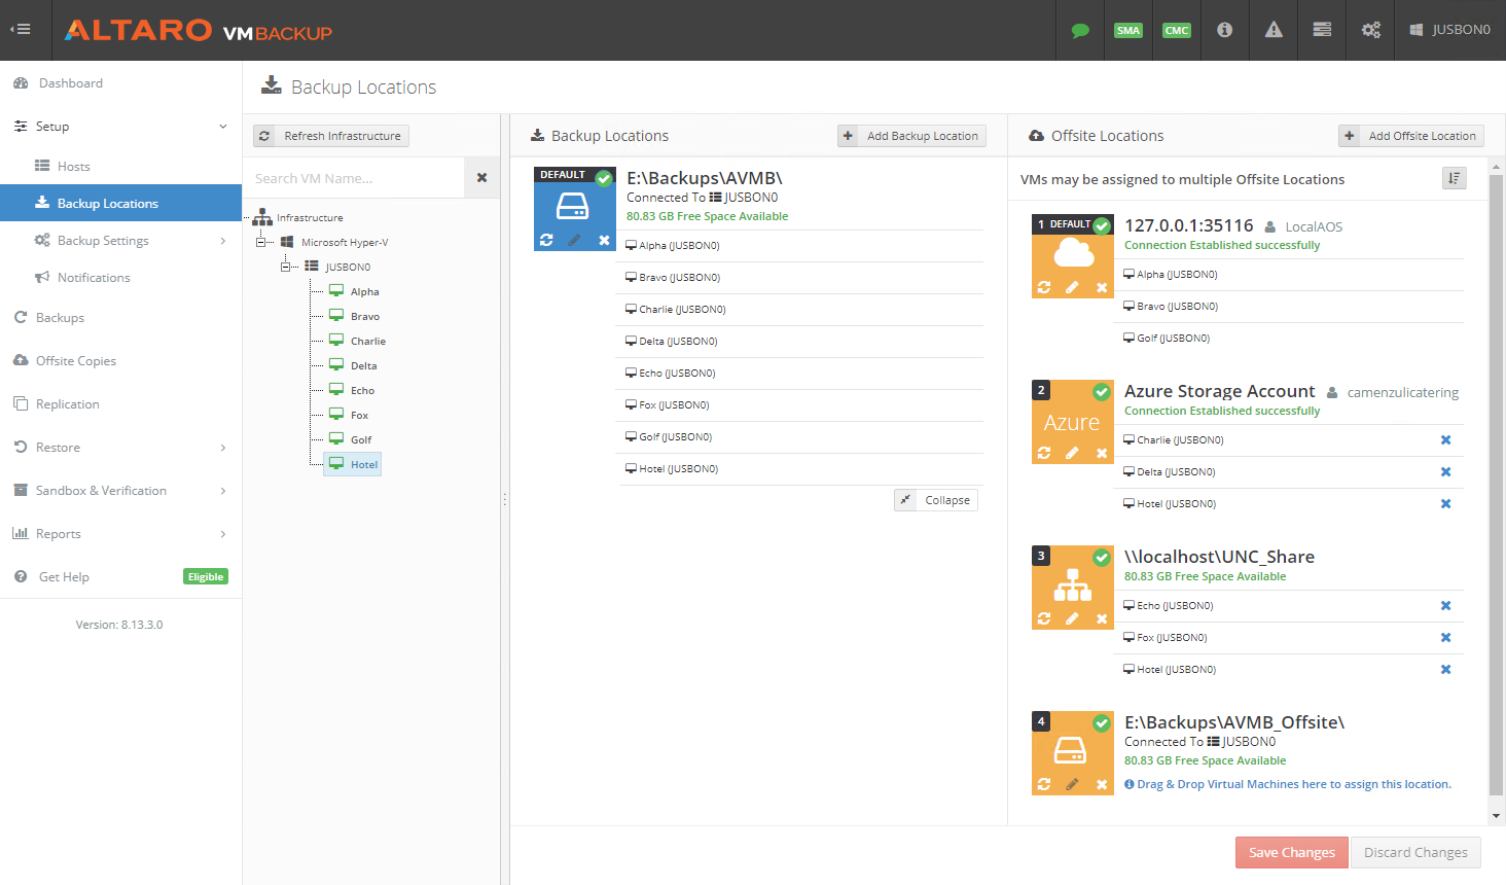
\includegraphics[width=15cm]{figures/backup-locations-big.png}
 \caption{Capture d'écran de la configuration des sauvegardes}
 \label{fig:altaro_back}
\end{figure}
Il suffit de configurer des sauvegardes, vers un support (physique, externe, off-site, etc..) hormis des cassettes, comme le montre la capture d'écran ~\ref{fig:altaro_back}. \newline
Sur cette capture d'écran, on voit un lieu en local, sur le lecteur E du serveur, ainsi que quatre lieux hors site, comprenant un cloud Azure, des serveurs locaux et des répertoires. \newline
Ensuite, il ne suffit plus que de faire un glisser déposer des serveurs vers les règles voulues.\newline
Ce moyen de configuration est plus pratique que Veeam et est accessible aux nouveaux utilisateurs. \newline
J'ai pu remarquer qu'Altaro se fonde sur la règle 3-2-1 copies, qui consiste en : \newline
\begin{itemize}
 \item Trois copies effectuées ;
 \item Sur deux supports différents ;
 \item Au moins une est externalisée. \newline 
\end{itemize}
Il n'est donc pas possible d'installer Altaro pour faire de l'externalisation uniquement, il faudra au préalable effectuer une copie en local. \newline
Une fois que le paramétrage est finalisé, les sauvegardes se font de manière automatique, à l'heure planifiée. Lorsqu'un job de sauvegarde est finalisé, Altaro s'occupe du suivi de l'état de celui ci. \newline
\begin{figure}[ht]
 \centering
 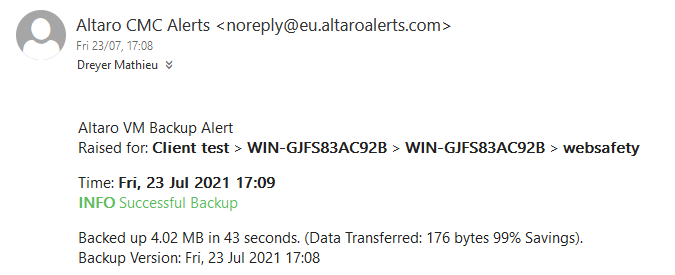
\includegraphics[width=12cm]{figures/mail altaro.png}
 \caption{Exemple de notification par mail pour suivre l'état des sauvegardes}
 \label{fig:altaro mail}
\end{figure}

En effet, après chaque sauvegarde, l'outil de sauvegarde envoie un mail aux différents responsables avec l'état de la sauvegarde, la durée de celle-ci et le type (locale, externalisée). \newline
Dans la capture d'écran ~\ref{fig:altaro mail}, il s'agit d'une sauvegarde effectuée en local, comme il n'y a pas la mention "off-site". \newline
Sur chaque serveur se trouvent les informations des sauvegardes.
\begin{figure}[ht]
 \centering
 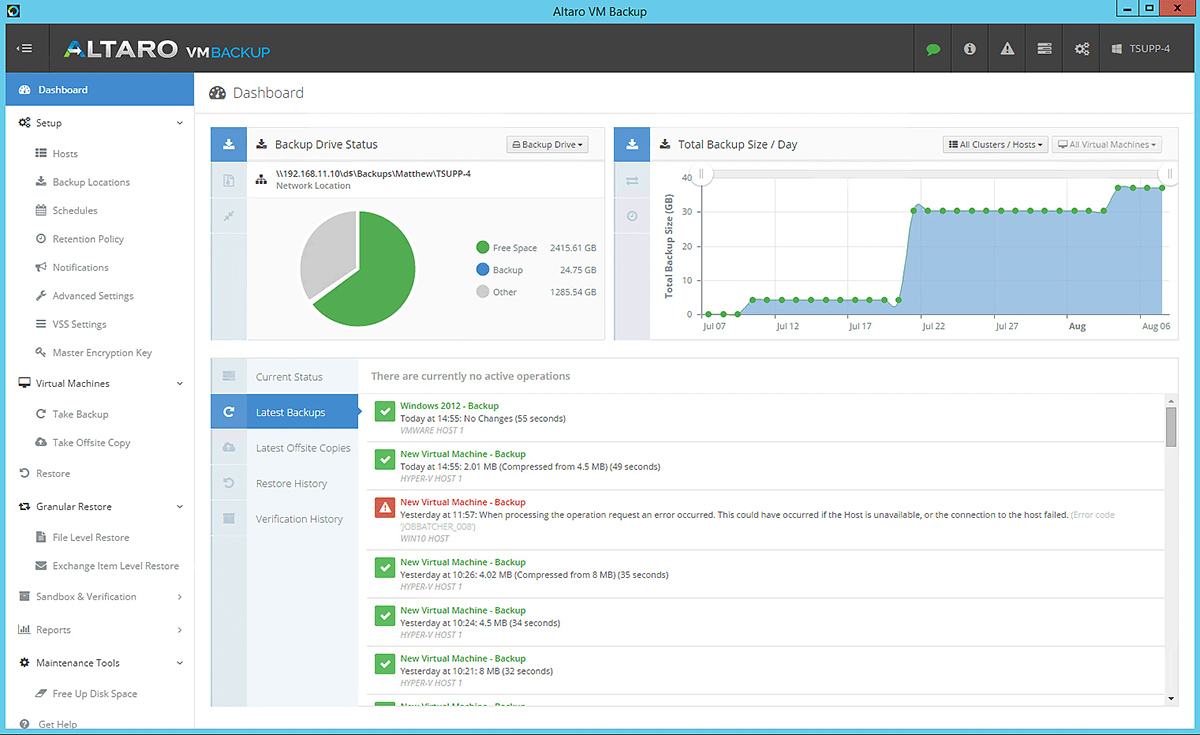
\includegraphics[width=15cm]{figures/Altaro-VM-Backup-dashboard.jpg}
 \caption{Capture d'écran de l'application Altaro VM backup}
 \label{fig:altaro console1}
\end{figure}

Sur la capture d'écran ~\ref{fig:altaro console1}, on peut voir l'espace nécessaire pour les sauvegardes. Cela permet de pouvoir anticiper une erreur due à un manque d'espace. L'application permet également d'avoir un journal d'évènement de l'ensemble des machines virtuelles gérées par ce serveur. \newline
Parmi les fonctionnalités nécessaires, nous remarquons que la solution propose une restauration granulaire de serveur de messagerie, ce qui est un point important pour nos clients. \newline
De plus, Altaro propose une console en ligne, qui permet d'avoir un retour sur l'ensemble des serveurs sauvegardés.

\begin{figure}[ht]
 \centering
 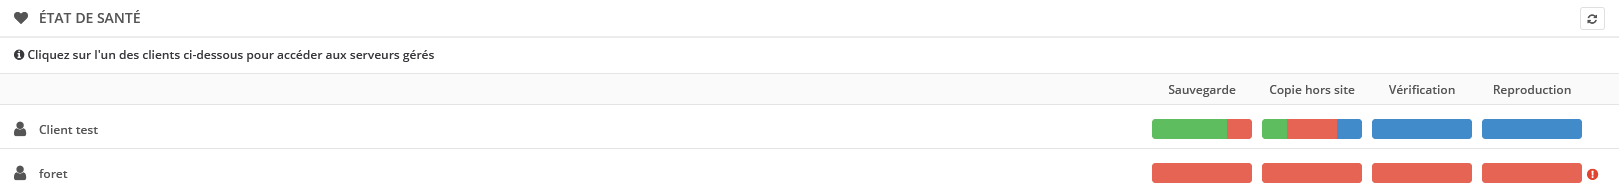
\includegraphics[width=15cm]{figures/etat sauvegarde.png}
 \caption{Capture d'écran de la console Altaro}
 \label{fig:altaro console}
\end{figure}
Sur la capture d'écran ~\ref{fig:altaro console}, on peut voir deux clients qui ont été créés. Le code couleur est le suivant : \newline
\begin{itemize}
 \item Vert : La sauvegarde s'est effectuée sans erreur;
 \item Rouge : La sauvegarde ne s'est pas effectuée, elle a recontré un problème;
 \item Bleu : L'hôte ne présente pas de sauvegarde configurée. \newline
\end{itemize}
Grâce à cette console, il est donc possible de voir rapidement où se situent les problèmes de sauvegarde, sur quel hôte et de pouvoir y remédier. \newline
A l'issue de la semaine de sauvegarde, j'ai simulé une attaque qui rend l'hôte injoignable. \newline

\begin{figure}[ht]
 \centering
 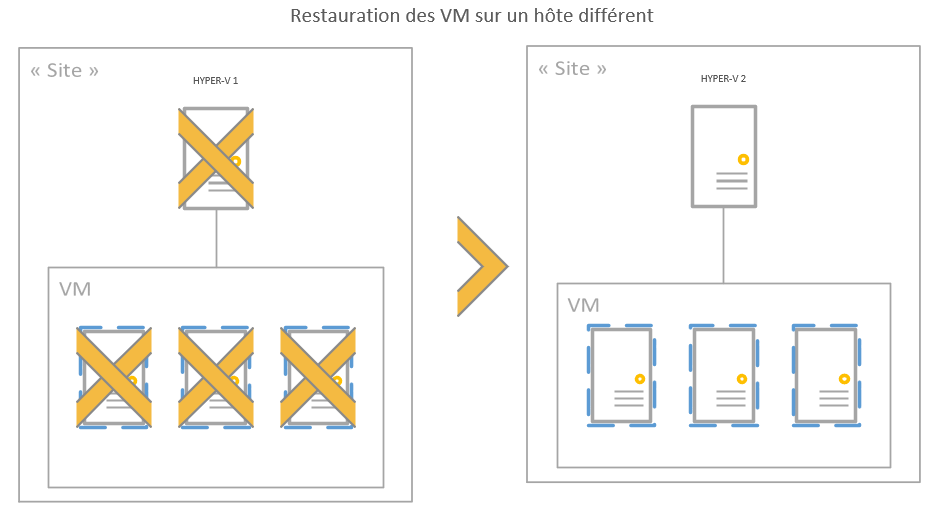
\includegraphics[width=15cm]{figures/restauration.png}
 \caption{Restauration sur un hôte différent suite à un dysfonctionnement}
 \label{fig:restau}
\end{figure}


Ceci permet de tester la restauration des différents serveurs, à partir d'un hôte différent, comme le représente le schéma ~\ref{fig:restau}. \newline
Il faut donc pouvoir restaurer l'ensemble des serveurs virtuels de manière à ne pas laisser le client bloqué. \newline
Un second serveur hyper-V a été installé avec l'agent Altaro. Ensuite, le serveur a été ajouté à la configuration du serveur hors site. \newline
J'ai pu remarqué au cours des tests qu'Altaro est compatible avec Windows Server 2012, mais qu'il dépend de PowerShell avec une version supérieure ou égale à  la 5.1. \newline 
Pour une installation de cet outil vers des anciens serveurs, il faudra donc vérifier les mises à jours et installer la version nécessaire.\newline
Tous les serveurs ont pu être restaurés et de manière rapide. \newline
Cependant, Altaro ne propose qu'un type de sauvegarde et ne prend pas en compte tout les supports. Il est alors intéressant de questionner sur la possibilité d'installer Altaro en mode hybride, avec Veeam comme solution de sauvegarde en local et Altaro en hors site. \newline
Comme Altaro nécessite un agent pour le fonctionnement, celui ci permet également de faire de la supervision. \newline
Il est possible de configurer des alertes en cas de déconnexion d'un serveur, d'espace disque saturé. 

\begin{figure}[ht]
 \centering
 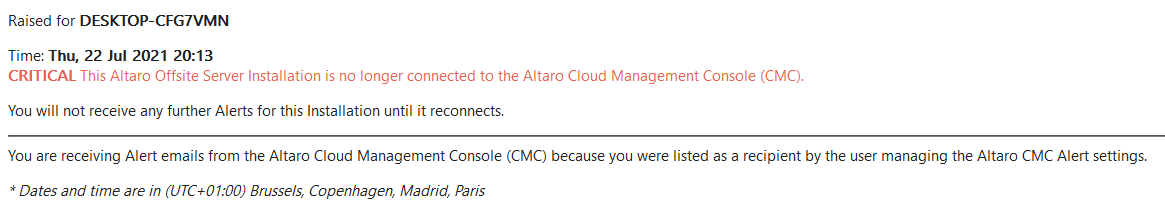
\includegraphics[width=15cm]{figures/mail altaro offline.png}
 \caption{Exemple de notification suite à un serveur indisponible}
 \label{fig:offline}
\end{figure}


\subsection{Test des temps de récupération et de sauvegarde}

Pour réduire au maximum le temps d'arrêt des clients, il est nécessaire de connaître les temps de restauration et de sauvegarde d'Altaro. \newline
Avec les serveurs de sauvegarde et le serveur hors site, des opérations de récupération et de sauvegarde ont été effectuées et chronométrées. Les tests ont été réalisés avec la fibre sur chaque serveur. \newline

\begin{table}[!h]
 \centering
 \begin{tabular}{|p{4cm}|p{2.5cm}|p{2.5cm}|p{2.5cm}|p{2.5cm}|}
 \hline & Restauration hors site & Restauration locale & Sauvegarde complète hors site & Sauvegarde complète locale\\
 \hline Données par minutes & 1.6Gb & 4Gb & 2Gb & 10Gb \\
 \hline 
 \end{tabular}
 \caption{Tableau comparatif des temps de restauration et de sauvegarde}
 \label{tab:temps}
\end{table}
Le tableau \ref{tab:temps} permet d'avoir une idée du temps moyen de récupération et de sauvegarde des données avec l'outil Altaro. Les temps sont corrects et permettent de ne pas bloquer un client de manière trop longue. \newline

\subsection{Avantages et inconvénients}

Suite aux différents tests, il est possible de voir les limites de Altaro et ses avantages.
Par rapport aux autres solutions qui sont bien positionnées sur le marché, celle ci se révèlent moins chéres, mais avec moins d'options. \newline
Elle est plus adaptée pour les petites structures, ou celles qui possèdent un serveur par fonctionnalité. Pour la sauvegarde des serveurs, il n'y a pas de restriction de système d'exploitation sur les machines virtuelles.
Altaro permet de faire des sauvegardes hors site, en se fondant sur la règle du 3-2-1 copies, avec une protection supplémentaire contre les virus. Les restaurations sont rapides également. \newline
D'un autre côté, la solution n'offre pas l'ensemble des fonctionnalités de Veeam, ce qui peut être un point de blocage pour certains clients. \newline 
Le manque de compatibilité avec les supports de types LTO est également à prendre en compte, sachant qu'une partie des clients fonctionne encore avec des cassettes. \newline
Une autre limite de la solution se trouve sur les serveurs avec plusieurs rôles et également sur les serveurs particuliers demandant une restauration granulaire. \newline
Enfin, il faut noter rigoureusement la clé de cryptage qui permet de restaurer les serveurs. \newline

\subsection{Utilisations possibles}

La solution peut être mise en place dans deux cas de figure. \newline
Le premier est en solution secondaire à Veeam, avec une copie hors site des sauvegardes. Il faut cependant disposer d'un espace de stockage pour les sauvegardes. En effet, Altaro copie une sauvegarde hors site, il faut donc au préalable une sauvegarde du serveur. \newline
La seconde possibilité est de mettre Altaro comme unique solution de sauvegarde. Avec les éléments précédents, il faut que les serveurs disposent d'un rôle uniquement. \newline
En conclusion, pour les clients de LMI, la solution Altaro s'adapte plus aux petits clients, qui possèdent un serveur physique avec des machines virtuelles. Il est préférable que chaque serveur virtuel possède un seul rôle.
\newpage

\section{Compatibilité entre les clients et Altaro}

Comme la solution présente des aspects négatifs qui sont bloquants, j'ai décidé de faire une analyse des clients et des besoins de ces derniers. \newline
Quatre clients ont été choisis comme référence suite à différents échanges avec la partie technique. Ces clients possèdent tous une particularité, qui se retrouve chez d'autres clients. \newline
Ainsi, il sera possible de définir au sein de quel type de structure, d'infrastructure la solution peut être mise en place. \newline

\subsection{Client 1}

\begin{figure}[ht]
 \centering
 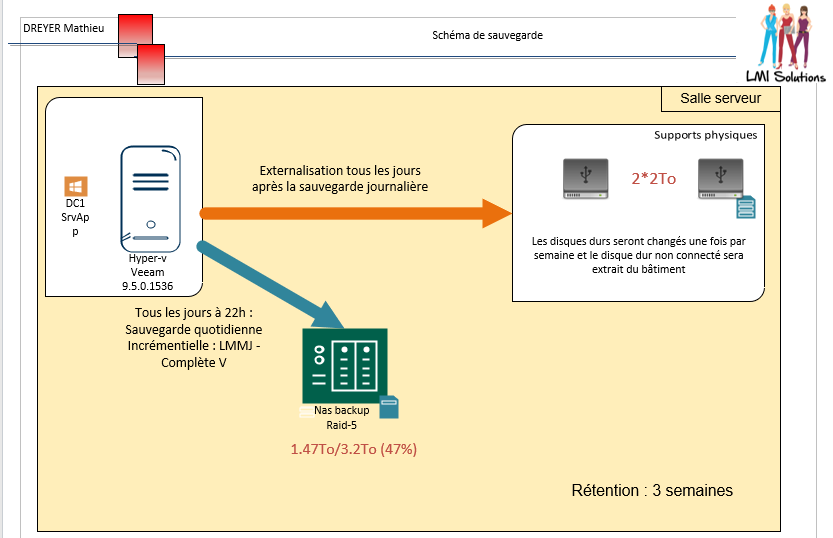
\includegraphics[width=15cm]{figures/client1.png}
 \caption{Infrastructure du client 1}
 \label{fig:client1}
\end{figure}
La figure \ref{fig:client1} illustre l'état des sauvegardes chez le client. \newline
Il s'agit d'une sauvegarde incrémentielle effectuée chaque jour à 22 heures. La sauvegarde est copiée sur deux supports, un nas et des disques durs externes. \newline
Le premier client possède l'infrastructure suivante : \newline
\begin{itemize}
 \item Un serveur physique;
 \item Deux serveurs virtuels (un contrôleur de domaine et serveur de fichier, un serveur applicatif) ;
\item Cinq postes clients avec une volumétrie de fichiers de 25 Go ;
\item Un serveur métier avec base de données HyperFiles SQL. \newline
\end{itemize}
On remarque que l'un des serveurs virtuels dispose de deux rôles, ce qui peut être compromettant pour Altaro. Il est nécessaire de planifier un rendez vous avec le client afin de définir des temps d'arrêt, des temps de reprise acceptables afin de savoir si la solution peut être mise en place. \newline
La sauvegarde actuellement mise en place est la suivante : 


Une réunion avec le client a été effectuée, afin de connaître les différents éléments à sauvegarder. Suite à l'échange, différentes informations ont pu être fournies : \newline
\begin{itemize}
 \item Le client souhaite sauvegarder uniquement ses serveurs ;
 \item La durée d'arrêt maximale est d'une demi journée ;
 \item Le client ne travaille pas sur des données importantes, donc il accepte de perdre jusqu'à une demi-journée de données en cas de dysfonctionnement. \newline
\end{itemize}

Suite à cette réunion, j'ai rédigé un schéma permettant de proposer au client un renouvellement de son outil de sauvegarde. 
\begin{figure}[ht]
 \centering
 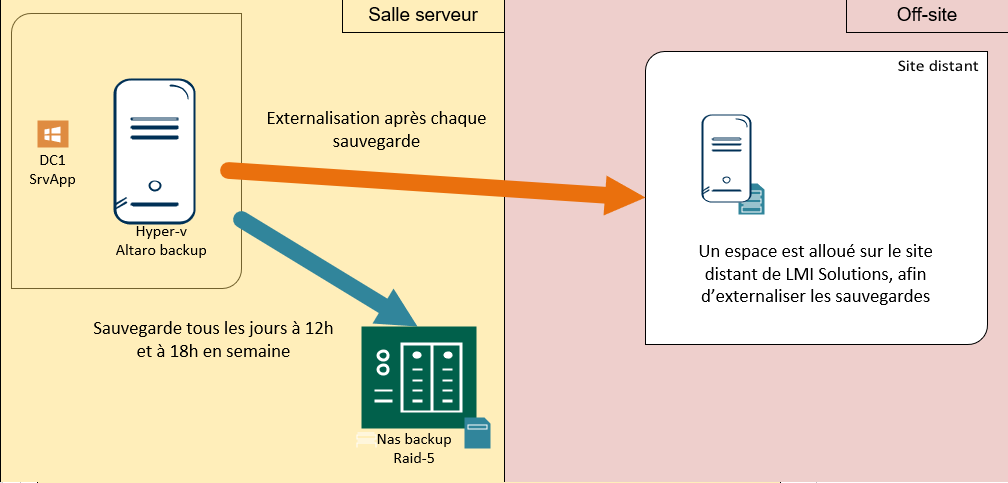
\includegraphics[width=15cm]{figures/client1_after.png}
 \caption{Infrastructure du client 1 avec Altaro}
 \label{fig:client1_altaro2}
\end{figure}
Le changement sur les sauvegardes est représenté sur la figure  \ref{fig:client1_altaro2}. Le but est de remplacer les supports amovibles par un point hors site, s'assurant que les sauvegardes soient bien dans un autre site. \newline
Veeam est facturé au client 200€ par an. La solution adaptée ici est Altaro avec le modèle MSP à 4.5€ par machines virtuelles, ce qui fait un total de 108€ par an. \newline
L'avantage pour le client est que la solution est moins coûteuse, les besoins du clients sont respectés et une partie de ses sauvegardes se trouvera à LMI Solutions, ce qui permet d'avoir un plan de relance en cas de perte du site. \newline
Une seconde réunion a été effectuée avec le client, Alexandre Petitcolas et moi-même afin de valider le changement. \newline
Comme LMI Solutions ferme les deux premières semaines d'août, la solution sera installée après cette période.

\subsection{Client 2}

Le second client possède l'infrastructure suivante : \newline
\begin{itemize}
 \item Un serveur physique 
 \item Trois serveurs virtuels (contrôleur de domaine / messagerie exchange / serveur de fichier) ;
\item Huit postes utilisateurs avec une volumétrie de 300 Go de fichier ;
\item Un serveur de messagerie de 85 Go. \newline
\end{itemize}

La sauvegarde actuellement mise en place est la suivante et est similaire à celle du premier client, à savoir une sauvegarde journalière en dehors des heures d'activité de l'entreprise. 
\begin{figure}[ht]
 \centering
 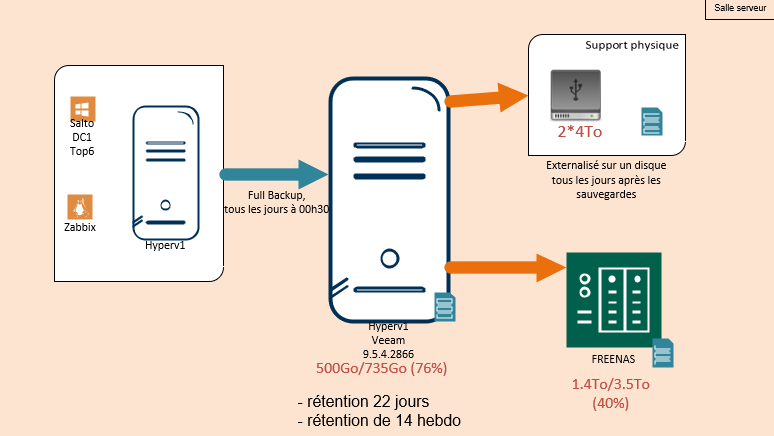
\includegraphics[width=15cm]{figures/client2.png}
 \caption{Infrastructure du client 2}
 \label{fig:client2}
\end{figure}
Chez ce client, comme le montre le schéma \ref{fig:client2}, les sauvegardes sont effectuées sur un serveur, puis sont copiées sur deux supports, un NAS et des disques durs. \newline
L'infrastructure du client semble compatible avec Altaro. Après un point avec L'équipe technique qui a confirmé ces informations, une réunion a été planifiée avec le client et l'équipe technique pour connaître les besoins et présenter la nouvelle installation possible. \newline
L'installation proposée est identique à celle du client 1 sur le schéma ~\ref{fig:client1_altaro2}, une sauvegarde sur un NAS local et une copie hors site. \newline
L'intervention d'installation et de configuration de l'outil sera planifiée également après la période de fermeture.
\subsection{Client 3}

Le troisième client possède l'infrastructure suivante : \newline
\begin{itemize}
 \item Un serveur physique ; 
 \item Quatre machines virtuelles (contrôleur de domaine / serveur de fichier / RDS / Serveur métier) ;
\item Cinq postes clients avec une volumétrie de fichiers de 25 Go ;
\item Un serveur métier Sage avec SQL Server;
\item 15 PCs sur deux sites distants (connexion des utilisateurs sur RDS), soit des fichiers totaux de 450 Go et une base SQL de 10 Go.\newline
\end{itemize}

La sauvegarde actuellement mise en place est la suivante : 
\begin{figure}[ht]
 \centering
 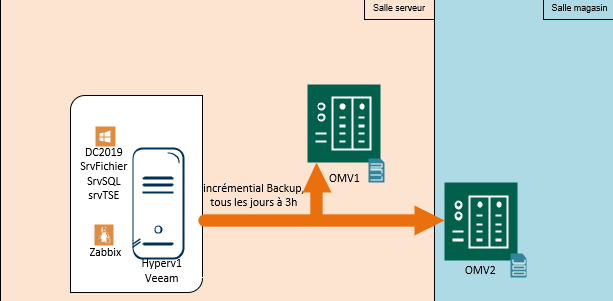
\includegraphics[width=15cm]{figures/client3.png}
 \caption{Infrastructure du client 3}
 \label{fig:client3}
\end{figure}
elle est constituée d'un serveur de sauvegarde, qui copie les données sur deux NAS, dont un qui se situe dans un autre local. \newline
Le schéma \ref{fig:client3} représente la mise en place actuelle. \newline
Une réunion a été planifiée avec le client pour connaître les différentes contraintes. 
Lors de la réunion, le client a évoqué le fait que de ne pas pouvoir revenir sur les données d'il y a quelques heures est bloquant pour lui, sachant qu'il y a souvent ce genre d'opérations, dû a de mauvaise manipulations ou plantage de l'applicatif métier. \newline
Bien que chaque serveur ait un rôle distinct, il n'est pas envisageable de basculer sur Altaro complètement pour ce client. \newline
De plus, il possède déjà une copie vers un site distant, ce qui permet d'avoir toujours accès à ces données. \newline
Le client 3 n'aura donc pas de modification de solution de sauvegarde.

\subsection{Client 4}

Le quatrième client possède l'infrastructure suivante : \newline
\begin{itemize}
 \item Deux serveur physique;
 \item Six serveurs virtuels (contrôleur de domaine / serveur de fichier / serveur de paie / serveur metier / rds / exchange) ;
\item 35 ordinateurs, 700 Go de données, base SQL pour paie et Base Oracle pour applicatif métier;
\item 180 Go de messagerie. \newline
\end{itemize}

La sauvegarde actuellement mise en place est la suivante : 
\begin{figure}[ht]
 \centering
 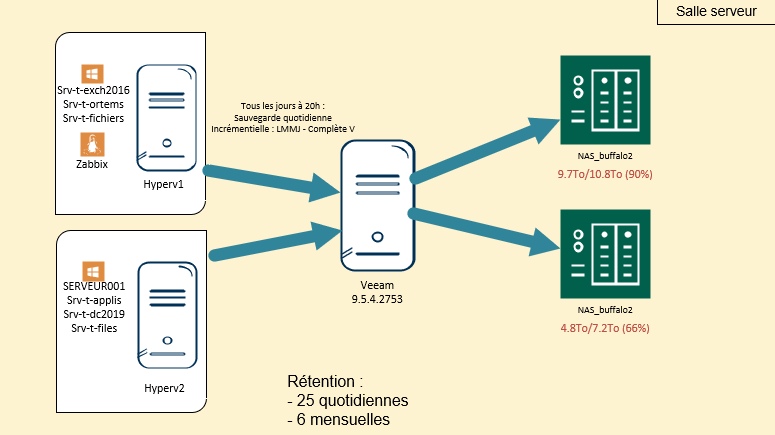
\includegraphics[width=15cm]{figures/client4.png}
 \caption{Infrastructure du client 4}
 \label{fig:client4}
\end{figure}
elle est composée de deux gestionnaires de serveur. Comme l'illustre le schéma \ref{fig:client4}, les données sont sauvegardées sur deux NAS, dans le même local. \newline
Cependant, en effectuant un point avec la partie technique, celle-ci m'a informé que les postes utilisateurs sont également sauvegardés chez ce client. \newline 
L'outil propose une solution de sauvegarde granulaire pour les mails, avec des serveurs exchange ou office 365. \newline
Altaro se situe principalement sur les serveurs et n'est pas compétitif sur la sauvegarde de postes. \newline
La solution n'a donc pas été proposée au client. \newline
Il serait cependant utile de mettre en place une sauvegarde externalisé avec Veeam, ou de mettre un des supports sur un autre site, pour augmenter la protection des sauvegardes. \newline

\subsection{Généralisation}

Avec les analyses des différents clients précédentes, il est possible de distinguer un type d'entreprise pour laquelle Altaro est adaptée. \newline
D'abord, il est nécessaire que l'entreprise n'ait pas à sauvegarder ses postes utilisateurs, comme la fonction n'est pas encore présente sur l'outil. \newline
Ensuite, dans le cas ou le client possède moins de 5 machines virtuelles, le modèle MSP est intéressant et moins cher. Dans le cas contraire, les offres unlimited seront plus adaptées. \newline
Enfin, la compatibilité dépendra du type de serveur et du rôle de chacun. Altaro offre une restauration granulaire sur une grande partie des serveurs, sauf sur les serveurs de type active directory ou SQL. \newline Il est donc préférable que ces serveurs possèdent un unique rôle. Cela permet de faire une sauvegarde de manière plus fréquente des machines virtuelles concernées et de les restaurer en cas de problème. \newline
Pour les déploiements futurs, l'idéal est de le faire de manière générique.

\begin{figure}[ht]
 \centering
 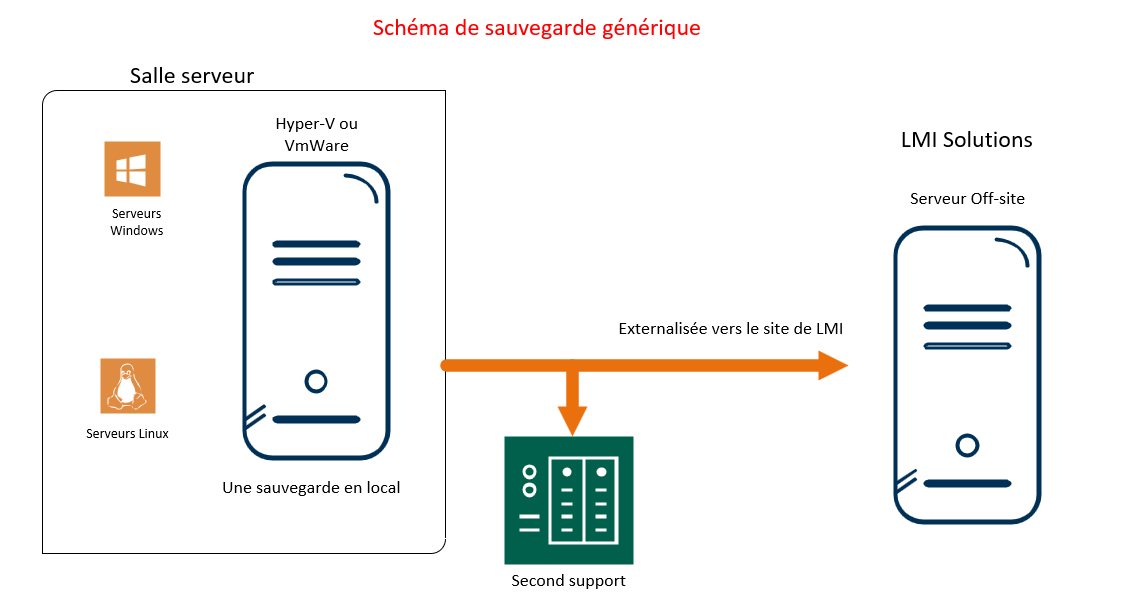
\includegraphics[width=17cm]{figures/générik.png}
 \caption{Infrastructure générique avec Altaro}
 \label{fig:generik}
\end{figure}

Comme le représente le schéma \ref{fig:generik}, le but est de faire trois copies, sur deux supports différents, avec une qui est externalisée. Ce type d'infrastructure est bénéfique pour le client et pour LMI Solutions, car en cas de panne d'un serveur, il est possible de restaurer rapidement. Et dans l'hypothèse d'une attaque virale, il suffit de restaurer les sauvegardes qui sont externalisées et donc qui ne sont pas infectées.

\section{Mise en place}

L'équipe technique a été missionnée sur la mise en place sur deux des clients. \newline
Comme je suis alternant, l'objectif est que la solution soit utilisés par les différents acteurs des sauvegardes et qu'ils la maîtrisent sans avoir besoin de mon aide. \newline
En effet, il faut que la solution soit utilisable par l'entreprise pour qu'elle apporte une plus value. \newline
Le but du projet étant de trouver une solution sur le long terme et mon contrat finissant le 31 août, il faut que l'équipe soit autonome avec cet outil. \newline  
Il a été nécessaire de former les différentes personnes sur l'outil.

\subsection{Transfert de compétences}

Afin que la mise en place se fasse dans les meilleures conditions, une demi journée de formation a été bloquée à LMI Solutions au profit des deux personnes affectées aux sauvegardes. \newline
J'ai rédigé un diaporama pour les accompagner au maximum sur la solution et les fonctions présentes. \newline
Ensuite, le serveur hors site ne change pas, il n'a pas été réinstallé. \newline
J'ai ensuite pris deux serveurs et j'ai accompagné les acteurs sur l'installation et la configuration. \newline
En plus de cette formation, j'ai rédigé une procédure d'installation afin d'aiguiller les personnes qui n'étaient pas présentes et également en cas de questionnement pour les personnes présentes. \newline 

\subsection{Plan de sauvegarde}

Il est essentiel pour le client de posséder un plan de sauvegarde. \newline
Un plan de sauvegarde reprend les informations suivantes : \newline
\begin{itemize}
 \item Objectif et périmètre, description de l'équipe ;
 \item Liste du matériel, données qui sont sauvegardées ;
 \item Calendrier des sauvegardes (dates, heures, fréquences) ;
 \item Liste des supports sur lesquels les données sont sauvegardées ;
 \item Définition des méthodes de sauvegarde ;
 \item Liste des tests et récurrence de ces derniers. \newline
\end{itemize}

Il permet aux clients d'avoir connaissance de tout ce qui est sauvegardé, à quelle fréquence. \newline

Cela permet en cas de panne, de savoir ce qui est récupérable et le temps d'arrêt. \newline
J'ai rédigé un plan de sauvegarde de manière générique et ce plan sera modifié et adapté pour chaque client. \newline
Ce document devra être mis à jour à chaque test, nouvelle sauvegarde ou modification de la configuration chez le client. \newline
Une réunion a été effectuée pour valider ce plan de sauvegarde et le présenter à l'équipe technique.

\section{Déploiement}

L'équipe technique est donc intervenue au sein de deux clients pour mettre en place Altaro. \newline
J'étais disponible en agence afin d'assurer le support en cas de problème. \newline
Après chaque installation, une vérification sera effectuée. \newline
La vérification portera sur l'ajout à la console dans un premier temps. Il faut s'assurer que les différents serveurs soient bien monitorés. Ensuite il faut vérifier les règles de sauvegardes, afin qu'elles correspondent aux besoins du client. \newline
Le plan de sauvegarde doit être modifié pour correspondre aux règles mises en place. \newline
Il faut également vérifier que les serveurs possèdent une copie hors site le lendemain de la mise en place. \newline
Enfin, les différents serveurs ont été ajoutés à la console de management. \newline
Au cours d'un projet, il est courant de faire face à des points bloquants. La prochaine partie traitera donc de ces éléments et les différentes actions mises en place afin de réussir à avancer dans le projet.

\clearpage

\chapter{Problèmes rencontrés et solutions}

Au cours de la réalisation de ce projet, j'ai rencontré différents problèmes. \newline
Premièrement, je n'avais pas eu l'occasion de travailler sur les sauvegardes de données avant ce projet. Il m'a donc fallu me renseigner sur ce domaine, qui m'était inconnu.
Ensuite, la communication a été difficile à mettre en place, étant donné que c'était l'un des premiers projets sur lequel je me suis retrouvé en autonomie. \newline
J'avais du mal à savoir quand échanger avec l'équipe et à trouver le moment opportun.
Un point a été effectué avec mon tuteur académique et mon tuteur d'entreprise. Il m'a permis de mieux comprendre les attendus du projet et comment mettre en place une communication plus adaptée. \newline
A l'issue de ce point, une gestion de projet plus rigoureuse a été mise en place, les documents que j'ai réalisés ont été mis sur le cloud de l'entreprise, permettant à toute l'équipe d'accéder aux différents travaux. \newline
Le projet a demandé beaucoup d'investissement. Au début du projet, comme le sujet m'était vague, je me suis renseigné sur le fonctionnement des sauvegardes. \newline
Cette tâche m'a pris plus de temps que prévu et j'ai dû moduler mon planning pour réussir ce projet. \newline
LMI Solutions m'a fourni le temps nécessaire au projet, en limitant mes autres missions, ce qui m'a permis de me consacrer pleinement au projet. \newline 
Grâce à cela, le projet a pu aboutir, avec une meilleure communication. \newline
De plus, avec la crise sanitaire que nous rencontrons actuellement, les demandes des clients sur la mise en place du télétravail ont augmenté. Les locaux de LMI Solutions ont permis d'accueillir l'ensemble de l'équipe, avec la mise en place du respect des gestes barrières et de distanciation sociale. Grâce à ces adaptions, il a été possible de se retrouver sur site afin de faire avancer le projet convenablement. \newpage

\section{Axes d'améliorations}

Comme nous l'avons vu, la solution Altaro est utile pour certains clients, avec une infrastructure définie, mais ne permet certaines fonctions essentielles. \newline
Certains serveurs, par exemple avec un applicatif métier particulier ne peuvent pas être restaurés de manière granulaire. Dans certains domaines, il est impossible de perdre une demi journée de travail.
Un axe d'amélioration serait de demander au fournisseur de l'applicatif métier d'effectuer un dump de la base. \newline
Il s'agit de faire une copie binaire brute d'une partie ou de la totalité d'un système de fichiers. \newline
Les dumps seraient faits de manière régulière en fonction du client. Par exemple, pour un client qui accepte une perte d'activité maximale sur deux heures, le fournisseur effectuera des dumps automatiques toutes les deux heures. \newline
Ceci permettrait d'avoir une sauvegarde par jour du serveur, sur lequel se trouveraient les différentes copies. Dans le cas où il faudrait restaurer le serveur, il sera alors possible de restaurer également l'application indépendamment du serveur. \newline
De plus, il est possible pour les clients possédant des cassettes de les accompagner vers une migration progressive de ce support. En effet, il est impossible de les supprimer du jour au lendemain. Par contre, il est possible d'introduire un autre support externe (disque dur, copie hors site), afin de compléter un cycle de rétention, pour ensuite supprimer les cassettes du processus. \newline
Enfin, il serait intéressant de mettre en place une externalisation hybride, vers deux types de supports différents. \newline
Cela permettrait d'avoir les données à LMI Solutions et également dans un cloud. Dans le cas où un problème surviendrait au sein de l'entreprise (coupure de courant, coupure internet), les sauvegardes resteront disponibles sur un cloud.\newline
Altaro est une solution qui est encore en développement, avec des nouvelles fonctionnalités qui se font de plus en plus nombreuses. \newline
La partie sauvegarde de serveur physique, ordinateur personnel est en train d'être renforcée. \newline
Des mises à jour seront déployées en septembre pour proposer ces fonctionnalités, avec des restaurations similaires à celles des machines virtuelles, ce qui permettra de pouvoir sauvegarder des postes utilisateurs. \newline
Il serait intéressant de suivre son évolution, afin de voir les nouvelles fonction qu'elle apportera.

\chapter{Conclusion}

Dans cette partie, il sera abordé une conclusion sur le projet au niveau de l'entreprise et à niveau personnel. Le but étant d'avoir connaissance des apports de ce dernier. Il est également intéressant de voir ce que m'a apporté le projet. 
\section{Pour l'entreprise}

Le projet à été valorisant pour l'entreprise. A travers celui-ci, une solution de sauvegarde qui apporte une réelle plus-value à l’entreprise a été mise en place, en réduisant certains coûts. \newline
Actuellement, un serveur est accessible à distance pour les futures copies hors-site. \newline
Dans le cas où Altaro ne serait pas mis en place chez tout les clients, il sera possible d'externaliser les sauvegarde depuis Veeam vers ce serveur. \newline
Cela permet d'éviter une rotation sur des disques durs externes, qui sont généralement stockés dans la pièce contenant le serveur de sauvegarde, ce qui réduit l'externalisation. \newline
De plus, ce projet à permis à l'équipe technique de se maintenir à jour sur les différentes solutions de sauvegarde existantes et de renforcer certains choix. \newline
Avec la crise sanitaire et les différents besoins des clients, les différents membres du projet n'ont pas toujours le temps de faire de la veille technologique. \newline A travers ce projet, ils connaissent les différents outils porteurs actuellement disponibles sur le marché. \newline
De plus, avec les différents documents réalisés sur les clients, il sera plus facile d'intervenir chez un client sans connaître son infrastructure au préalable. \newline
Enfin, il est maintenant plus simple pour les responsables des sauvegardes de suivre l'état des ces dernières avec le nouvel outil. Le programme développé peut également être rattaché à Altaro, ce qui permet d'avoir le retour sur la console en ligne, et le mail avec l'état général des sauvegardes en prenant en compte les deux outils. \newline
Les éléments principaux de la problématique ont été traités. 
Pour les futurs clients, l'entreprise pourra facilement définir la solution à mettre en place, avec l'analyse qui a été effectuée. \newpage

\section{A titre personnel}

J’ai acquis de nouvelles compétences, telles que mon autonomie au travail ainsi que mes capacités à communiquer avec l'équipe.\newline
Ce projet m'a permis de mettre en application les différentes notions de gestion de projet apprise au cours de mon cycle de formation et à m'adapter aux entreprises. Avant ce projet, je ne connaissais que les grandes lignes des sauvegardes. Maintenant je comprend les intérêts et les enjeux qu'elles représentent pour les entreprises. 
LMI Solutions m'a fait confiance en m'accordant ce projet qui a un réel avantage pour les clients et pour l'entreprise. Le fait d'avoir été accompagné et suivi par mon tuteur académique et mon maître d'apprentissage a été bénéfique. Ainsi j'ai réussi à définir le projet, à le réaliser et à faire des retours réguliers aux différents acteurs. \newline
LMI Solutions est une petite structure, avec l'ensemble des collaborateurs sur place. Une communication a été mise en place et maintenue tout au long du projet grâce à la proximité des différents acteurs. \newline
J'ai pu mettre en place une gestion de projet et j'ai dû respecter des jalons. Avec le respect des livrables, le projet a pu aboutir. \newline
De plus, à travers ce projet et mes trois années d'alternance, j'ai découvert de nombreux outils dans diverses domaines, qui m'ont permis de mieux comprendre la gestion informatique au sein des entreprises. \newline
En effet, LMI Solutions m'a formé sur plusieurs domaines, tels que l'infrastructure, avec la gestion et la mise en place de celle-ci, le développement, dans différents langages avec des dates butoirs à respecter et enfin le réseau, qui comprend divers équipements. \newline
Le fait d'avoir fait mon alternance dans une société de service m'a aidé à mieux comprendre le fonctionnement des entreprises, à réagir rapidement en cas de problème. J'ai réussi à m'adapter pour changer de mission facilement en cas de pannes de réseau pour me rendre sur site, diagnostiquer et résoudre le(s) problème(s).
J'ai travaillé avec l'ensemble de l'équipe de LMI Solutions sur des sujets différents et ils m'ont toujours accompagné afin que je puisse ensuite résoudre le problème en autonomie.


\cleardoublepage

\listoffigures
\cleardoublepage

\listoftables
\cleardoublepage

\printglossary[type=\acronymtype]

\cleardoublepage
\renewcommand{\thesubsection}{\Roman{subsection}}

\appendix


\cleardoublepage
\thispagestyle{empty}

\section*{Résumé}
\addcontentsline{toc}{chapter}{Résumé}

Le projet qui m'a été confié concerne les sauvegardes informatiques. Ce rapport contient l'ensemble des démarches  afin de mettre en place un outil de sauvegarde qui permet l'externalisation et la centralisation des données. L'entreprise d'accueil pour mon alternance et pour mon projet étant LMI Solutions, société de service informatique. 

Le but de ce projet est de réfléchir à la mise en place d'une solution de sauvegarde adaptable aux différents besoins de LMI Solutions, mais également des différents clients.

Ce rapport présentera l'ensemble de la gestion de projet appliquée, avec les acteurs du projet ainsi que leurs rôles, les différentes phases de ce dernier et le travail réalisé durant ces phases. Des axes d'amélioration du projet seront également présentés, dans le but de rendre le projet viable sur le long terme. 



{\bf Mots-clés : Sauvegarde, Externalisation, Gestion de projet}


\section*{Abstract}
\addcontentsline{toc}{chapter}{Abstract}

The project I have been assigned concerns computer backups. This report contains all the steps to set up a backup tool that allows the outsourcing and centralisation of data. The host company for my work placement and for my project is LMI Solutions, an IT service company. 

The aim of this project is to think about the implementation of a backup solution that can be adapted to the different needs of LMI Solutions, but also of the different clients.

This report will present the whole project management applied, with the actors of the project and their roles, the different phases of the project and the work done during these phases. In addition, areas for improvement will be presented, with the aim of making the project viable in the long term. 


{\bf Keywords : backup, centralisation, projet management }

\end{document}
